\chapter{Desenvolvimento} \label{cap:desenvolvimento}

Devido à importância do tema e ao raciocínio apresentado, um método para análise de \index{Vulnerabilidade}vulnerabilidades em redes industriais \index{OPC UA}OPC UA foi desenvolvido. O presente capítulo oferece os principais aspectos da bancada experimental utilizada e o conjunto de estratégias adotados para a realização e desenvolvimento do mesmo.

\section{Aspectos da Bancada Experimental para Ensaios de Intrusão em Redes OPC UA}

    Nesta seção, toda a estrutura responsável pela aquisição de dados experimentais gerados para auxiliar no desenvolvimento do trabalho é descrita. A \autoref{fig:esqBanc} ilustra a composição da estrutura da bancada experimental utilizada, cujos principais componentes são detalhados a seguir:

    \begin{figure}[htbp]
        \caption{\label{fig:esqBanc}Esquema geral da bancada experimental para ensaios de segurança cibernética}
        \begin{center}
            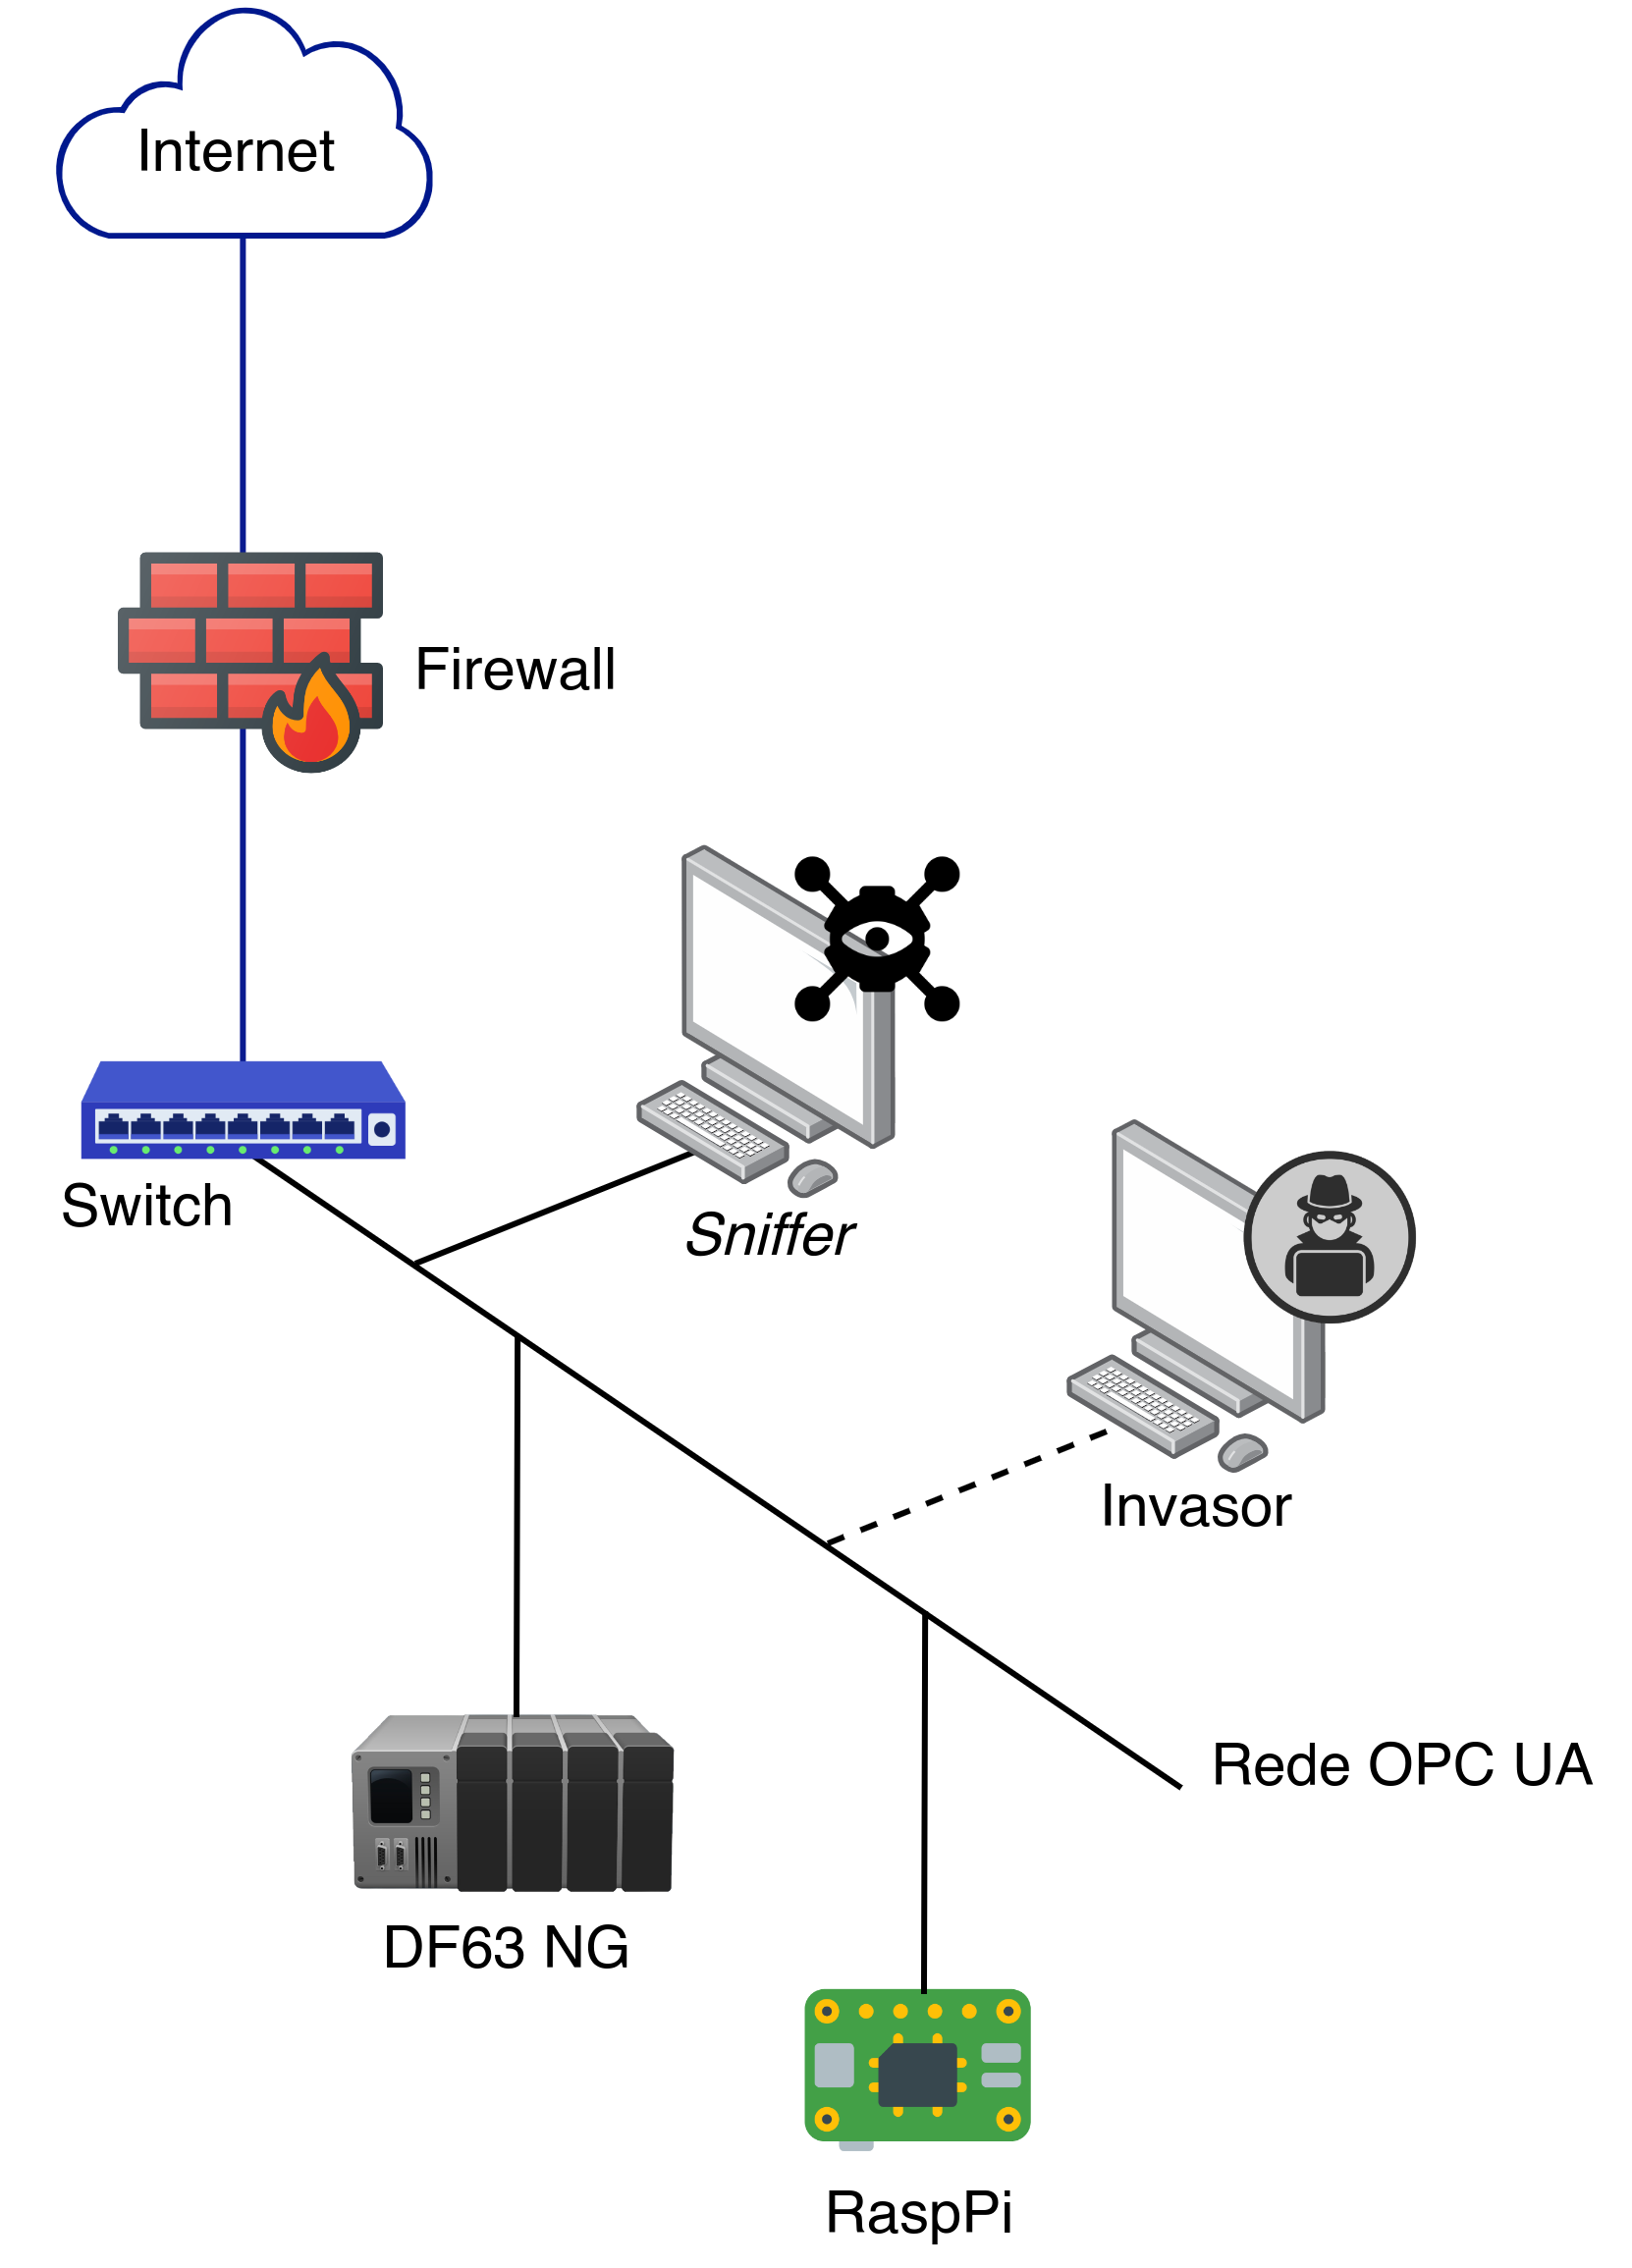
\includegraphics[width=0.6\textwidth]{USPSC-img/bancada.png}
        \end{center}
        \legend{Fonte: elaborada pelo autor.}
    \end{figure}

    \subsection{\textit{Hardware}}

    Para simular os ataques cibernéticos, são necessários um conjunto de componentes de \textit{hardware} combinados com ferramentas de \textit{software} específicas. A lista a seguir detalha cada equipamento utilizado.

    \begin{itemize}
        \item \underline{DF63 NG}: representa a nova geração dos controladores multifuncionais da plataforma DFI302 da Nova Smar S/A funcionando como um `\textit{linking device}' para conectar redes H1 independentes e redes Ethernet HSE, especialmente projetado para soluções de controle distribuído em redes industriais. Além de suportar comunicação Modbus, oferece recursos avançados, incluindo redundância `\textit{Hot standby}', comunicação OPC UA nativa, estampa de tempo e configuração por meio da linguagem Ladder conforme IEC 61131. A DF63 NG é altamente versátil, permitindo a instanciação de centenas de blocos funcionais, incluindo blocos flexíveis, e possui um servidor Web integrado para diagnóstico e parametrização;
        \item \underline{Raspberry Pi 4 Modelo B}: são utilizados dois mini-computadores de placa única multiplataforma, configuradas com o sistema operacional Kali Linux, hospedando um cliente e um servidor OPC UA cada. A Raspberry Pi 4 Modelo B representa uma evolução significativa em relação às gerações anteriores, incorporando um processador ARM Cortex-A72 quad-core de 64 bits rodando a 1,5 GHz, suporte a Wi-Fi 802.11ac, Bluetooth 5.0 e maior capacidade de memória. Estes aprimoramentos garantem um ambiente experimental mais robusto e capacidade de processamento aprimorada para a condução de testes de intrusão em redes OPC UA. Todas as Raspberry Pi's existentes na bancada experimental são configuradas como cliente e servidor OPC UA;
        \item \underline{Ethernet Switch}: Trata-se de um dos dispositivos de rede mais ubíquos, empregado para centralizar a comunicação entre múltiplos dispositivos. Utiliza a técnica de comutação de pacotes para receber e encaminhar dados de um dispositivo para outro. Neste projeto, faz-se uso de um \textit{Switch} Ethernet da marca TP-Link para estabelecer uma conexão entre os clientes OPC UA e o servidor. O componente de rede que atuar como hospedeiro do servidor OPC UA, encontra-se conectado ao comutador Ethernet por meio de um cabo LAN, da mesma maneira que outro responsável por hospedar o cliente também está conectado ao\textit{Switch}. Cumpre destacar que os comutadores Ethernet da TP-Link incorporam tecnologia Ethernet verde, que resulta em economia de consumo energético, enquanto o controle de fluxo IEEE 802.3x proporciona uma transferência de dados confiável.
        \item \underline{Elemento Invasor}: desempenha um papel fundamental na condução dos testes de intrusão propostos neste estudo. Representa uma simulação de ataque por meio de um computador que pode ser configurado de maneira flexível para atender a cenários específicos de teste. Os ataques são realizados utilizando uma variedade de ferramentas de software, como Hping3 e Nmap (veja \autoref{subsec:software}). Vale ressaltar que o Elemento Invasor é empregado com extrema cautela em um ambiente controlado, a fim de evitar qualquer impacto adverso e garantir a segurança contínua. Assim, respeitando rigorosamente as considerações éticas, os ataques efetuados neste trabalho pelo elemento invasor não implicam em nenhuma violação das regulamentações estabelecidas pela Lei Geral de Proteção de Dados (LGPD) por não ser aplicado em nenhuma rede ou implementação real.
    \end{itemize}
    
    \subsection{\textit{Software}} \label{subsec:software}

    Um conjunto de ferramentas de \textit{software} é necessário para conduzir os ataques às redes OPC UA, das quais se destacam:

    \begin{itemize}
        \item \underline{Smar OPC UA server}: servidor OPC UA proprietário da Nova Smar S/A, é amplamente aplicado no setor industrial juntamente com a linha de produtos compatíveis com o novo padrão O-PAS (do inglês, \textit{Open Process Automation™ Standards}), desenvolvido pelo OPAF (do inglês, \textit{Open Process Automation™ Forum}), oferecendo um ambiente altamente seguro e eficiente para a comunicação e troca de dados em sistemas de automação industrial. A Nova Smar S/A continua aprimorando seu servidor OPC UA para atender às crescentes demandas do mercado, proporcionando uma solução de conectividade sólida e confiável;
        \item \underline{opcua-asyncio}: implementação de código aberto do OPC UA, escrito em Python com suporte para asyncio. O opcua-asyncio opera sob a GNU Lesser General Public License v3.0,  permitindo sua integração e distribuição com \textit{software} proprietário. Essa biblioteca é versátil, compatível com vários ambientes Python, e oferece informações detalhadas sobre a implementação de clientes e servidor OPC UA. O opcua-asyncio implementa o conjunto de protocolos binários OPC UA, SDK de cliente e servidor, e é uma opção flexível para desenvolvedores que preferem Python como sua linguagem de programação;
        \item \underline{OPC UA Exploit Framework}: projeto \textit{open-source}, desenvolvido e mantido pela Claroty Team82, que fornece um framework avançado de ferramentas para pesquisa e exploração de vulnerabilidades em redes OPC UA. O intuito deste projeto é facilitar e auxiliar empresas desenvolvedoras de software e fornecedoras de OPC UA na fase de teste e aprimoramento dos seus produtos, além de suportar pesquisadores da área na análise de novas vulnerabilidades e \textit{bugs} sistêmicos;
        \item \underline{Ettercap}: ferramenta de \textit{software} utilizada principalmente para implementar ataques do tipo MITM. Possui recursos extras de captura de conexões \textit{real-time}, filtragem de conteúdo e análise de \textit{hosts} de destino. O Ettercap é utilizado neste projeto para implementar o primeiro cenário de ataque, capturando a conexão entre cliente e servidor OPC UA;
        \item \underline{Hping3}: ferramenta de linha de comando que serve como montadora e analisadora de pacotes TCP/IP. Inicialmente concebida para executar ataques de negação de serviço (DoS), o hping3 é agora amplamente empregado em testes de segurança de rede. Oferece suporte a protocolos TCP, UDP e ICMP, bem como um modo de rastreamento de rota;
        \item \underline{Wireshark}: software de código aberto usado para capturar e analisar pacotes e protocolos de rede. É principalmente aplicado para solução de problemas de rede, desenvolvimento e análise de protocolos de software e comunicação. Neste trabalho, é utilizado juntamente com um computador \textit{sniffer};
        \item \underline{Nmap}: ferramenta gratuita de código aberto amplamente utilizada para varredura de rede e portas. Através dela, pode-se descobrir os \textit{hosts} e serviços em uma rede dada, bem como detalhes como qual serviço está em execução em qual porta e se a porta está aberta ou fechada, entre outros. Esse resultado é alcançado ao enviar pacotes para o alvo e analisar posteriormente sua resposta.
    \end{itemize}

    A \autoref{fig:banc} apresenta a bancada experimental para ensaios de segurança cibernética.
    
    \begin{figure}[htbp]
        \caption{\label{fig:banc}Bancada experimental para ensaios de segurança cibernética}
        \begin{center}
            \includegraphics[width=0.5\textwidth]{USPSC-img/cyberkit2.png}
        \end{center}
        \legend{Fonte: elaborada pelo autor.}
    \end{figure}

\section{Ataques Cibernéticos em Redes Industriais OPC UA} \label{sec:attacks}

    Nesta seção, uma análise detalhada dos cenários de ataque implementados minuciosamente no âmbito deste projeto é apresentada. A exposição abrangente engloba uma descrição passo a passo das metodologias empregadas para orquestrar três formas distintas de ciberataques: intervenção de pacotes (do inglês \textit{Packet Sniffing}), ataques do tipo MITM e de negação de serviço. Ao elucidar as complexidades destes vetores de ataque, objetiva-se proporcionar uma compreensão profunda do cenário em evolução das ameaças à cibersegurança em redes OPC UA.

    \subsection{\textit{Packet Sniffing}}

    Uma vez que a rede OPC UA esteja instalada e funcionando em seus respectivos dispositivos, o Elemento Invasor inicia o \textit{software} Ettercap e o utiliza como um \textit{sniffer} unificado para obter informações detalhadas sobre os alvos disponíveis na rede. O modo unificado do Ettercap permite a execução do ataque por uma única interface de rede. É importante observar que o Elemento Invasor deve estar configurado na mesma rede de comunicação OPC UA e conectado a uma porta do \textit{switch} gerenciável, que por sua vez, replica o tráfego de dados das outras portas (do componente cliente e servidor OPC UA), conforme ilustrado na \autoref{fig:sniffing}. 

    \begin{figure}[htbp]
        \caption{\label{fig:sniffing}Esquemático do ataque \textit{Packet Sniffing}}
        \begin{center}
            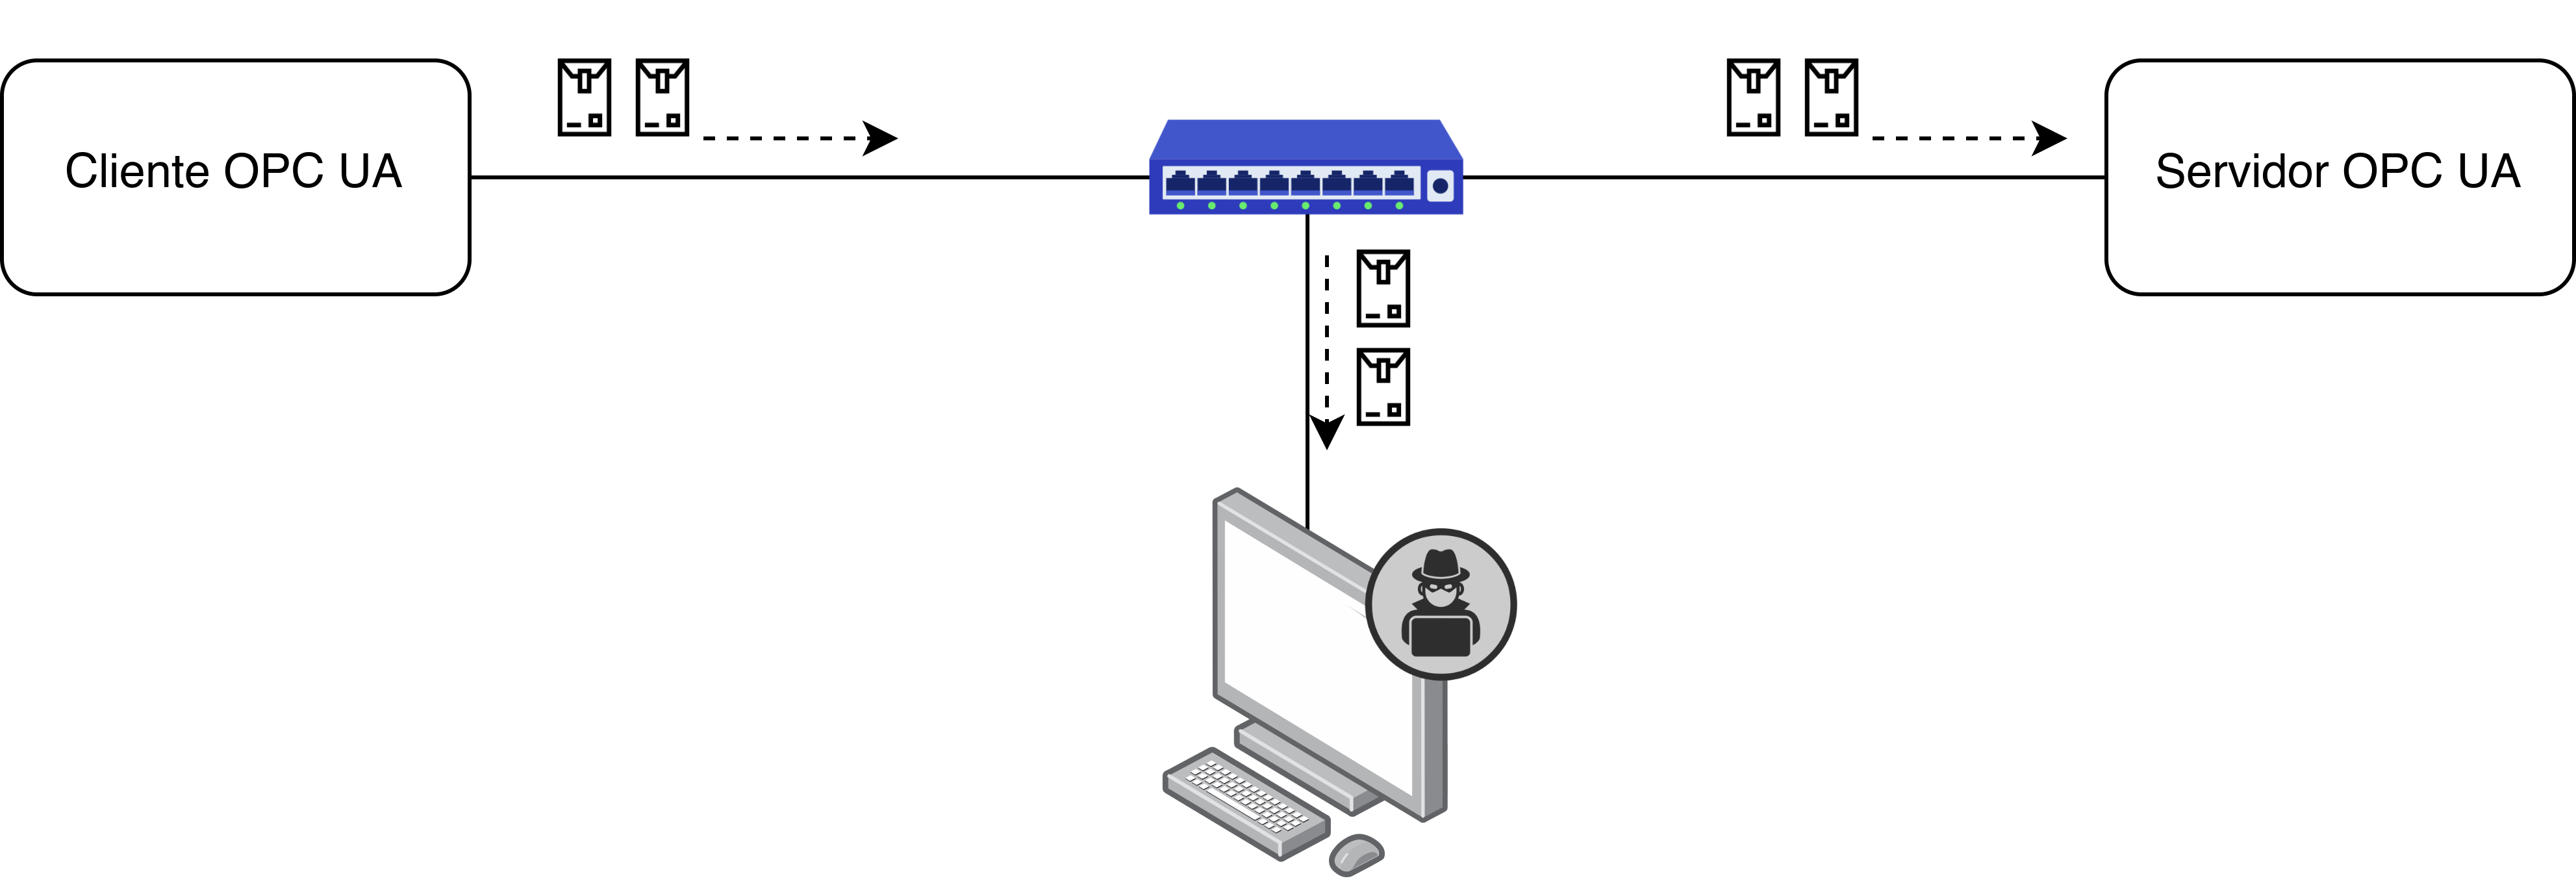
\includegraphics[width=0.9\textwidth]{USPSC-img/sniffing.png}
        \end{center}
        \legend{Fonte: elaborada pelo autor.}
    \end{figure}
    
    Com o \textit{sniffing} de rede iniciado pelo Ettercap, utiliza-se o Wireshark para analisar mais detalhes sobre os endereços obtidos. A \autoref{fig:sniffWire} apresenta a série de pacotes que o \textit{software} disponibiliza quando a operação de \textit{sniffing} do tráfego de rede é bem-sucedida. Maiores detalhes da análise aplicada nos dados obtidos nesse processo são apresentados no \autoref{cap:resultados}.

    \begin{figure}[htbp]
        \caption{\label{fig:sniffWire}Resultados de captura do Wireshark durante o \textit{sniffing} de pacotes}
        \begin{center}
            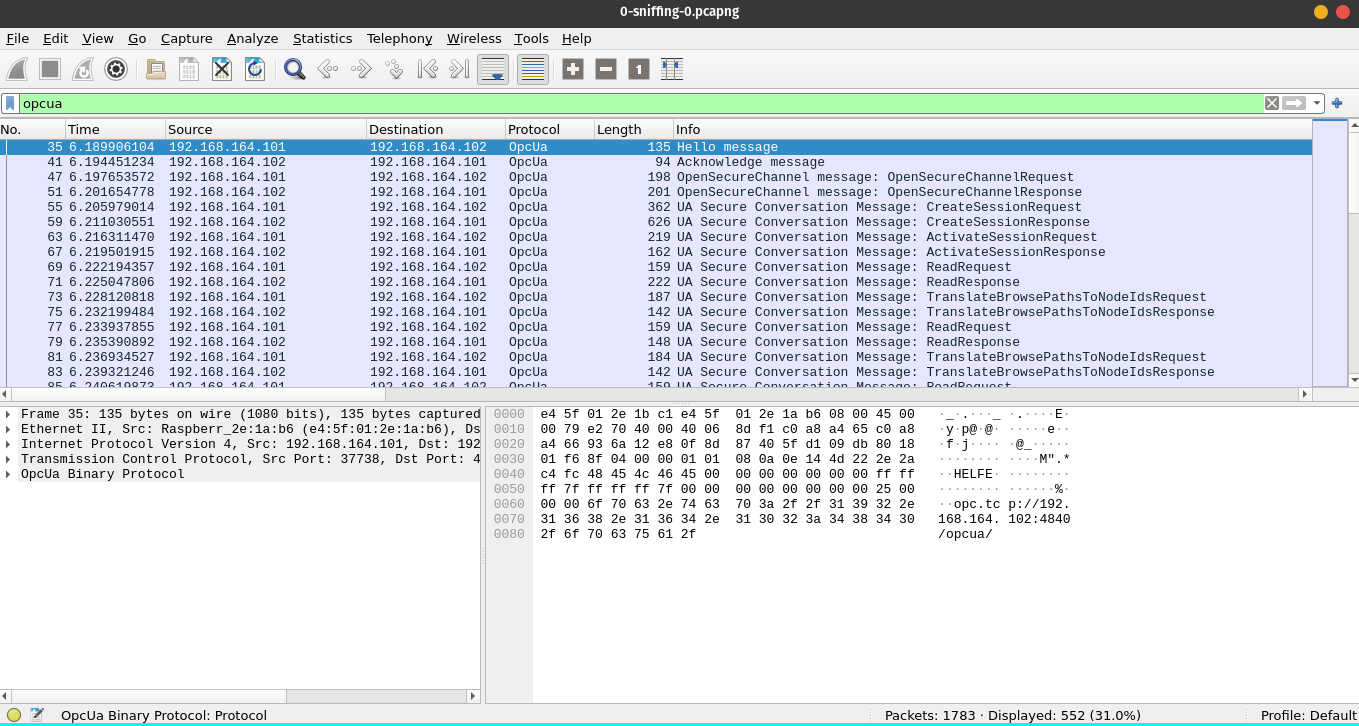
\includegraphics[width=1\textwidth]{USPSC-img/sniffWire.png}
        \end{center}
        \legend{Fonte: elaborada pelo autor.}
    \end{figure}
    
    Os detalhes dos pacotes capturados pelo Wireshark são analisados e descritos detalhadamente no \autoref{cap:resultados}.
    
    \subsection{\textit{Man in the Middle (MITM)}}

    Ao efetuar esse ataque, o Elemento Invasor pode interceptar as informações do \textbf{SecureChannel} entre o cliente e servidor OPC UA, como mostra a \autoref{fig:mitm}.

    \begin{figure}[htbp]
        \caption{\label{fig:mitm}Esquemático do ataque MITM}
        \begin{center}
            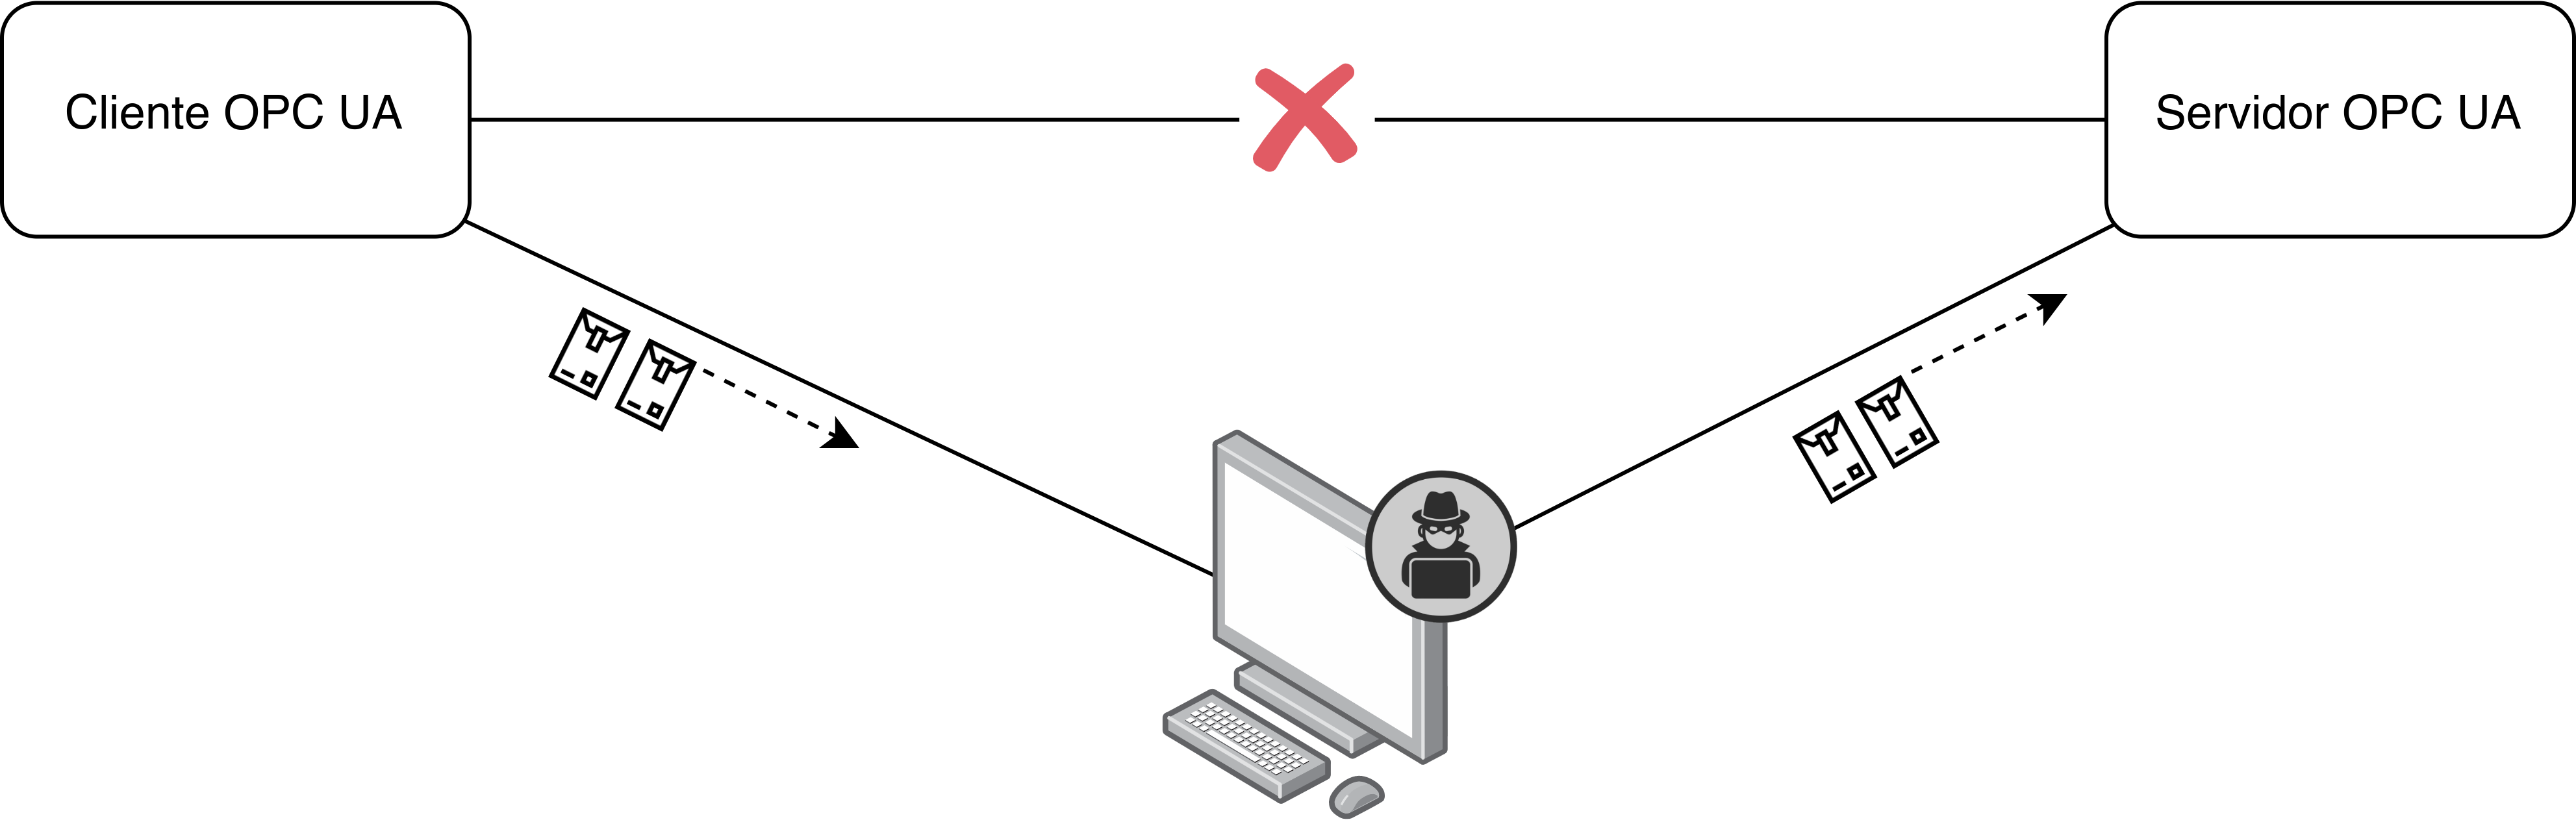
\includegraphics[width=0.9\textwidth]{USPSC-img/mitm.png}
        \end{center}
        \legend{Fonte: elaborada pelo autor.}
    \end{figure}
    
    A primeira ferramenta de software utilizada nesse processo é a Ettercap, utilizada para realizar uma varredura da rede. Ao iniciar a busca direta por \textit{hosts} ativos, todos os endereços da máscara de rede são verificados a fim de identificar quais deles estão em funcionamento. Como exemplo, caso a máscara de rede configurada seja 255.255.255.0 (24), um total de 256 endereços são varridos.
    
    Após o término dessa operação de varredura, o Elemento Invasor pode selecionar o(s) alvo(s) nos quais receberam o ataque MITM e então, prosseguir com a falsificação da rede por ARP (do inglês \textit{ARP Spoofing}), um dos tipos mais comuns de efetuar esse ataque. O ARP (do ingês \textit{Address Resolution Protocol}) é um dos protocolos de comunicação mais importantes da camada de rede do modelo OSI, utilizado para determinar o endereço MAC (do inglês \textit{Media Access Control}) de um dispositivo com base no seu endereço IP. Com o \textit{ARP Spoofing}, o invasor é capaz de anunciar à rede que o seu endereço MAC é o correto para os endereços IP pertencentes ao roteador e à estação de trabalho. Assim, estes dois dispositivos atualizam as suas entradas de cache ARP, e, a partir desse ponto, comunicam-se com o invasor, em vez de diretamente entre si.

    Enquanto a falsificação da tabela ARP é realizada pela ferramenta Ettercap, inicia-se a captura de pacotes pelo Wireshark. Para facilitar a visualização e a análise realizada neste estudo, o Wireshark é configurado para o protocolo OPC UA, permitindo um exame detalhado da comunicação entre os dispositivos na rede.
    
    \subsection{\textit{Denial of Service (DoS)}}

    Esse tipo de ataque possibilita a inserção de clientes não confiáveis na rede OPC UA pelo Elemento Invasor, assim como uma inundação da rede e do servidor ao enviar mensagens específicas continuamente. A \autoref{fig:dos} apresenta um esquemático básico de um funcionamento de DoS, nas quais as solicitações advindas de um cliente OPC UA não confiável são interpretadas pelo servidor, mas não são aceitas pelo remetente devido à sua falsificação de endereço.

     \begin{figure}[htbp]
        \caption{\label{fig:dos}Esquemático do ataque DoS}
        \begin{center}
            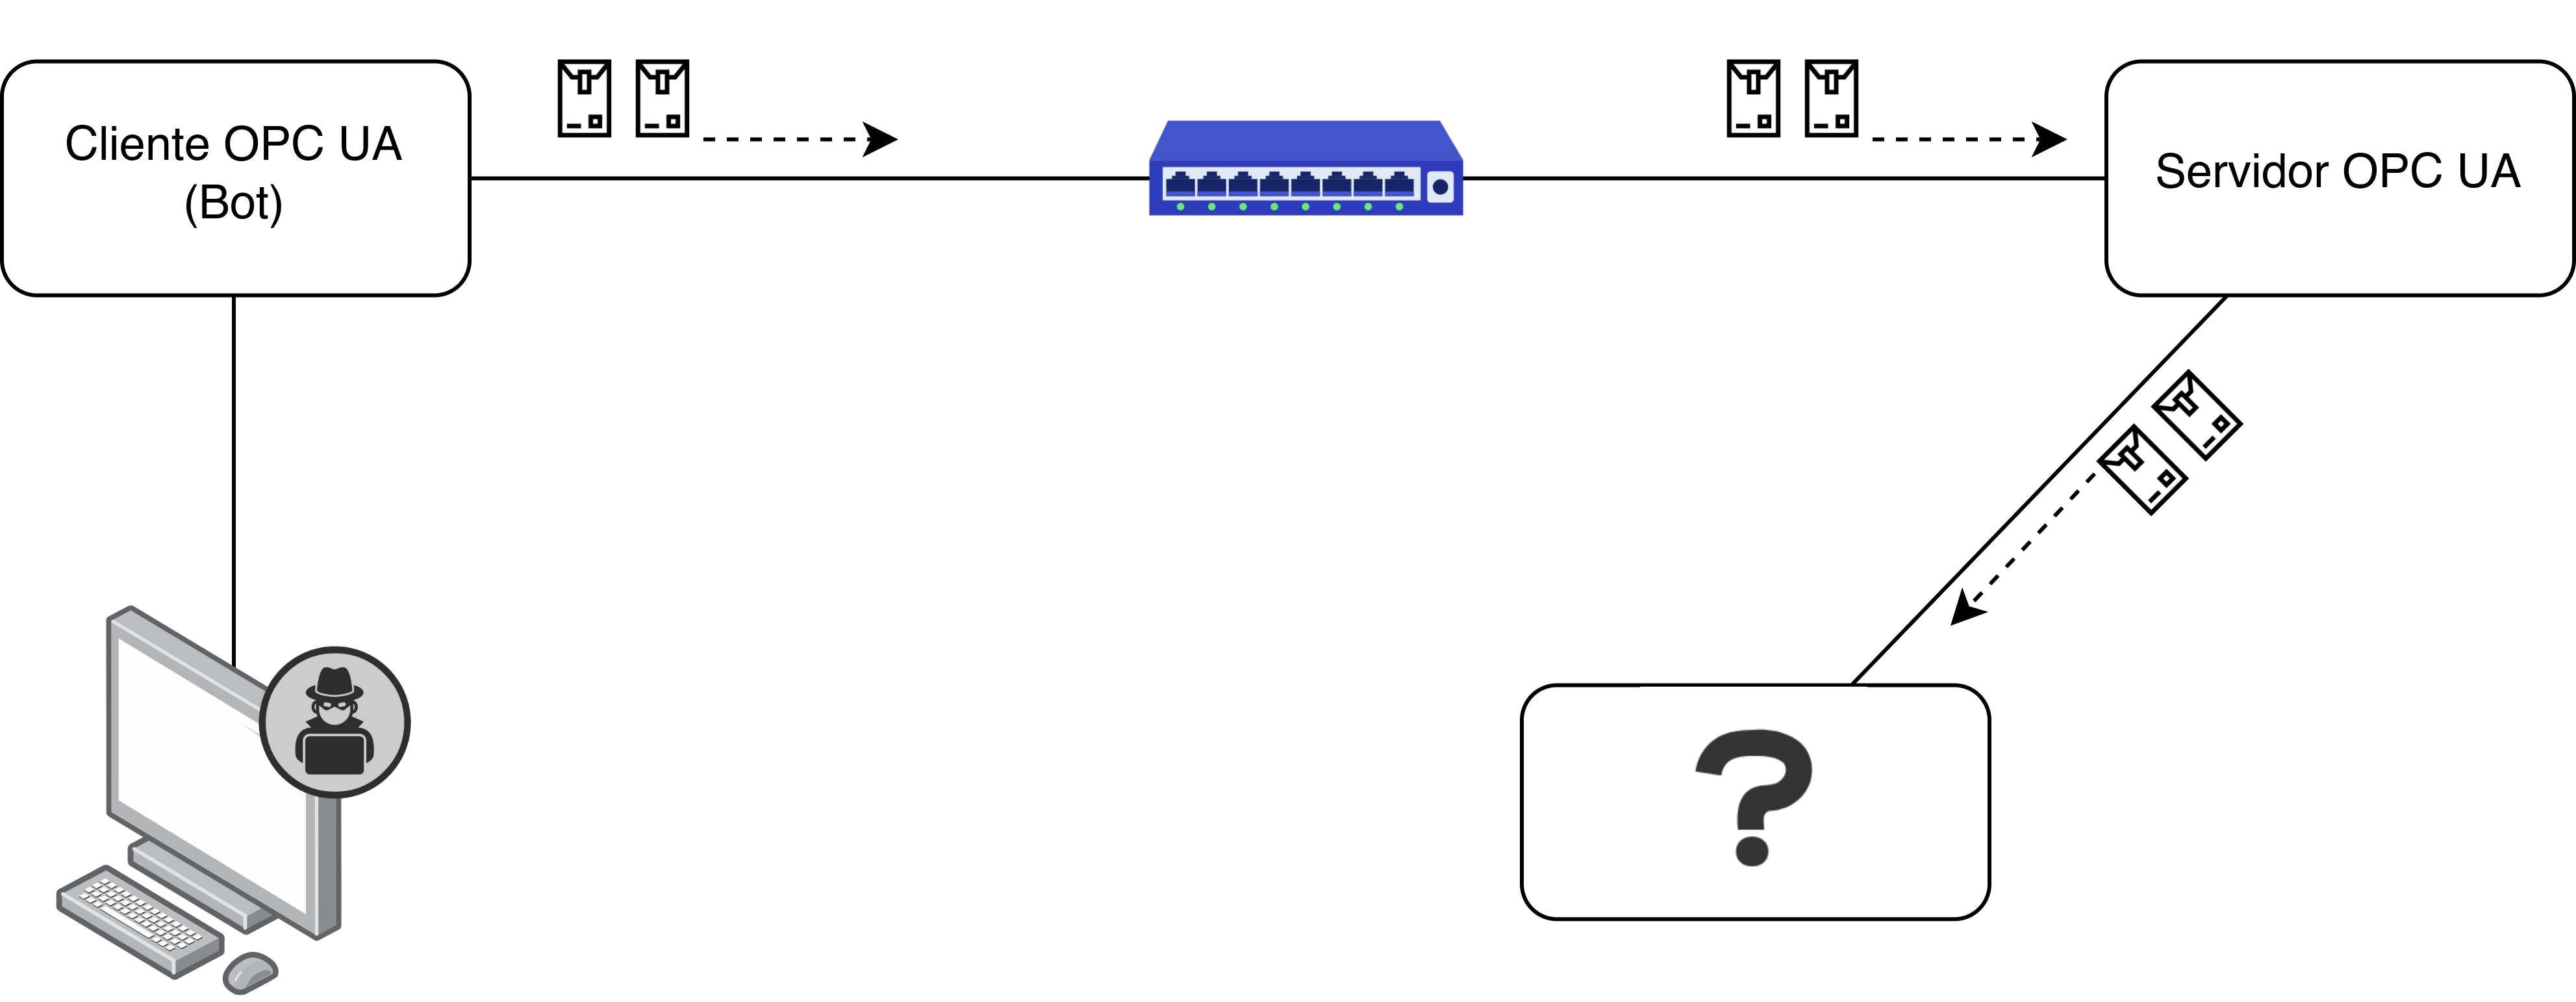
\includegraphics[width=0.9\textwidth]{USPSC-img/dos.png}
        \end{center}
        \legend{Fonte: elaborada pelo autor.}
    \end{figure}
    
    Existem diversos cenários possíveis para a efetuação do ataque de negação de serviço. Além do impacto da inundação na rede, ressaltam-se os efeitos no processamento do componente ao sofrer ataques intensivos, no qual o servidor precisa avaliar as certificações para responderem solicitações. Segundo \citeonline{neu2019}, os principais cenários são:

    \begin{enumerate}
        \item \underline{SYN \textit{Flooding}}: o cliente sobrecarrega o servidor enviando mensagens SYN de forma contínua, e o servidor responde com ACK a cada uma dessas mensagens. Embora essa ação possa inundar a rede com tráfego sobrecarregado com estas mensagens, seu impacto no consumo de recursos do servidor é limitado;
        \item \underline{ACK ou ERR \textit{Flooding}}: nesse cenário, o cliente inunda o servidor com mensagens ACK e/ou ERR, às quais o servidor responde com mensagens ERR. Da mesma forma do anterior, pode haver sobrecarga na rede, mas possui impacto moderado nos recursos do servidor;
        \item \underline{Inundação com Mensagens Incorretas}: são enviadas continuamente mensagens incorretas pelo Elemento Invasor, forçando respostas ERR pelo servidor. Também cria-se sobrecarga na rede, mas apresenta impacto relativamente baixo no processamento do servidor;
        \item \underline{CLO \textit{Flooding}}: enviam-se, repetidamente, mensagens de solicitação de fechamento de canal (CLO) ao servidor, que responde com mensagens ERR, sobrecarregando a rede com o tráfego destas mensagens.
        \item \underline{Inundação com \textbf{FindServers} ou \textbf{GetEndpoints}}: O cliente estabelece um canal no modo de segurança \textbf{None} e, em seguida, envia continuamente mensagens \textbf{FindServers()} ou \textbf{GetEndpoints()} para o servidor, que, por sua vez, responde com as mesmas mensagens por meio do OPC UA MSG. Apesar de apresentar impacto na rede, não altera os recursos do servidor;
        \item \underline{Inundação com Solicitações SYN e OPN}: um cliente não confiável realiza um ataque de negação de serviço enviando continuamente solicitações SYN e OPN ao servidor. O servidor responde com mensagens ACK e ERR. Nesse ataque, o servidor consome recursos substanciais durante a validação do certificado, na solicitação e no processo de criptografia da mensagem. Esse ataque pode ser ainda mais eficaz quando a Autoridade de Certificação está localizada em um sistema diferente, aumentando consideravelmente o tempo de validação do certificado, e, consequentemente, o processamento do componente onde se encontra o servidor.
    \end{enumerate}

    Duas ferramentas são utilizadas para efetuar a inundação da rede e, assim, alcançar o DoS: OPC UA Exploit Framework e Hping3, além de aplicar o Nmap para efetuar uma varredura da rede a fim de encontrar portas abertas e endereços IP disponíveis. 

    Uma vez que o Elemento Invasor obteve acesso a algum dos componentes da rede do alvo, o Nmap é utilizado para mapeamento da rede em questão. O comando abaixo executa um \textit{scan} SYN em um range de IPs, relativamente não-obstrusivo e camuflado, uma vez que ele nunca completa uma conexão TCP. Também chamado de escaneamento de portas entreabertas (\textit{half-open scanning}), um pacote SYN é enviado como se fosse abrir uma conexão real, cuja espera-se uma resposta. Um SYN/ACK indica que a porta está ouvindo (aberta), enquanto um RST (\textit{reset}) é indicativo de uma não-ouvinte. Se nenhuma resposta é recebida após diversas retransmissões, a porta é marcada como filtrada. A porta também é marcada como filtrada se um erro ICMP de inalcançável é recebido.

    \begin{minted}[
        breaklines,
        %linenos,
        mathescape,
        encoding=utf8,
        framesep=2mm,
        baselinestretch=1.2,
        bgcolor=codeback,
        fontsize=\footnotesize
    ]{console}
nmap -sS 192.168.164.*
    \end{minted}

    A correta execução desse mapeamento resulta em uma lista de IPs disponíveis e portas abertas, que servirão de entrada para os próximos passos. O Hping3 é utilizado para realizar o SYN \textit{Flooding} (1) na rede. Para isso, o \textit{script} de configuração abaixo deve ser implementado pelo Elemento Invasor, customizando-o de acordo com cada cenário.

    \begin{minted}[
        breaklines,
        %linenos,
        mathescape,
        encoding=utf8,
        framesep=2mm,
        baselinestretch=1.2,
        bgcolor=codeback,
        fontsize=\footnotesize
    ]{bash}
# CONFIGURAÇÃO
set TARGET "192.168.164.101"  # O alvo do ataque
set FAKEIP "192.168.164.201"  # Endereço falso
set BROADCAST "192.168.164.254"  # Endereço de broadcast da rede

set PORTS {{4840}{4192}}  # Utilizar as portas abertas encontradas no Nmap
set PORTUDP 123  # Utilizar uma porta UDP ativa

set commandRunTime 60

# EXECUÇÃO
foreach port $PORTS {
    lappend commands "hping3 -S -a $FAKEIP -p $port --flood -V $TARGET"
}
    \end{minted}

    Com isso, o Hping3 está preparado para iniciar o ataque direcionado ao endereço e portas especificados, com uma frequência predefinida (neste caso, sessenta segundos). A interpretação dos parâmetros utilizados na execução é a seguinte: o argumento \textbf{-S} define o tipo de ataque, \textbf{-p} identifica a porta de destino, \textbf{-V} indica o endereço IP do alvo, enquanto \textbf{-a} determina o endereço IP falsificado utilizado no ataque, uma estratégia que pode contornar \textit{firewalls} de forma eficaz.

    Por fim, alguns ataques mais robustos são efetuados com o auxílio da ferramenta OPC UA Exploit Framework. Os ataques de negação de serviço disponibilizados pelo \textit{framework} e escolhidos para execução no ambiente de simulação industrial proposto, são apresentados abaixo, seguidos de suas respectivas categorias, conforme os cenários supracitados e apresentados por \citeonline{neu2019}, e suas descrições:

    \begin{itemize}
        \item[N/A] \underline{Loop infinito na cadeia de certificados}: refere-se a uma situação em que algum servidor implementa a verificação da cadeia de certificados por conta própria, sem proteção contra um loop de cadeia infinita. Isso pode ocorrer quando um certificado A, por exemplo, é assinado por outro certificado B, que por sua vez é assinado pelo A. Cria-se uma dependência circular entre os certificados A e B, resultando em um loop infinito durante o processo de verificação da cadeia de certificados;
        % \item[(3)] \underline{Inundação por \textit{Chunk}}: envolve o envio de uma quantidade abundante de fragmentos de dados ao servidor sem o envio do fragmento final correspondente. O OPC UA permite a divisão dos dados em fragmentos, comumente chamados como \textit{MessageChunks} ou \textit{Chunks}, que são enviados à medida que são codificados, a fim de facilitar a transmissão e o processamento. Caso ocorra um erro na criação de um destes fragmentos, um \textit{Chunk} final deve ser enviado ao destinatário para notificar o erro, que por sua vez, é marcado com um sinalizador `A' (abortar) para indicar o erro. O receptor deve verificar a segurança do \textit{MessageChunk} abortado antes de processá-lo e, caso esteja tudo certo, ignorar a mensagem, mas sem encerrar o \textbf{SecureChannel};
        \item[(3)] \underline{Chamada da função \textit{Dereference} nula}: envolve a chamada de vários métodos OPC UA e encerramento da sessão antes da conclusão destes. Isso resulta em uma situação em que a aplicação servidora é forçada a referenciar um objeto nulo ou um ponteiro invalido, levando a um erro de execução;
        \item[(6)] \underline{Abertura de múltiplos canais seguros}: tentativa de inundação do servidor com uma quantidade abundante de solicitações \textbf{OpenSecureChannels};
        % \item[(3)] \underline{Mensagem aninhada complexa}: aplicação de uma variante especialmente manipulada e complexa, projetada para explorar vulnerabilidades em um servidor OPC UA. Quando esta variante é processada pelo servidor, ela pode causar um estouro na pilha de chamadas (\textit{call stack overflow}), levando a uma falha no servidor;
        \item[(5)] \underline{Tradução do caminho de navegação}: são enviadas ao servidor requisições de traduções de \textit{browse path} complexas que exploram a falta de limites adequados na resolução destes caminhos, podendo causar também um \textit{call stack overflow};
        % \item[Não aplicável] \underline{Falha de espera no \textit{Thread Pool}}: caracteriza uma paralisação (\textit{deadlock}) no sistema de \textit{Thread Pool} -- mecanismo de gerenciamento de \textit{threads} utilizado para processar solicitações de clientes e tarefas no servidor OPC UA -- devido à inanição simultânea de tarefas concorrentes. Em termos mais simples, quando vários processos ou \textit{threads} estão competindo por recursos do \textit{Thread Pools} de um servidor e, devido a problemas de sincronização ou gerenciamento inadequado de \textit{threads}, ficam em um estado de espera prolongado, impedindo efetivamente o servidor de processar solicitações legítimas;
        % \item[(6)] \underline{Persistência ilimitada de subscrições}: inúmeras solicitações de monitoramento ao servidor são enviados por um invasor, todas configuradas para não excluir os itens após o monitoramento. Esta persistência resulta em uma alocação descontrolada de recursos de memória pelo servidor, levando eventualmente a uma negação de serviço devido ao esgotamento de recursos.
        % \item[(3)] \underline{Chamada da função \textit{Dereference} nula}: envolve a chamada de vários métodos OPC UA e encerramento da sessão antes da conclusão destes. Isso resulta em uma situação em que a aplicação servidora é forçada a referenciar um objeto nulo ou um ponteiro invalido, levando a um erro de execução;
        % \item[(3)] \underline{Alteração de corrida e navegação no espaçamento de endereço}: o Elemento Invasor realiza a adição de \textit{Nodes} no \textit{Address Space} no servidor e, simultaneamente, remove-os em um ciclo contínuo, enquanto percorre todo o espaçamento de endereço. Esta manobra cria uma situação de competição na qual o servidor está sendo constantemente modificado e examinado ao mesmo tempo, podendo, assim, esgotar os recursos de processamento e resultar em problemas de consistência no \textit{Address Space};
        % \item[(6)] \underline{Atualização de condição ilimitada}: refere-se ao envio repetido e quantidade abundante de chamadas do método \textbf{ConditionRefresh}, o que leva a alocações de memória não controladas e, eventualmente, pode resultar em uma falha no sistema. O método ConditionRefresh é usado para atualizar as condições e estados das variáveis monitoradas em um servidor OPC UA.
    \end{itemize}

    Sabendo disso, os ataques acima podem ser efetuados através da seguinte linha de comando base, substituindo SERVER\_TYPE pelo tipo de servidor utilizado (\textit{e.g.}, softing, unified, prosys, kepware, triangle, dotnetstd, open62541, ignition, rust, node-opcua, opcua-python, milo e s2opc), IP\_ADDR pelo endereço de IP do alvo, PORT pela porta aberta para a comunicação UA, ENDPOINT\_ADDRESS pelo endpoint do servidor, FUNC\_TYPE pelo tipo de ataque escolhido (verificar na documentação oficial do framework quais os nomes das funções disponíveis \cite{claroty2023}) e DIR, necessário para algumas funções:

    \begin{minted}[
        breaklines,
        %linenos,
        mathescape,
        encoding=utf8,
        framesep=2mm,
        baselinestretch=1.2,
        bgcolor=codeback,
        fontsize=\footnotesize
    ]{console}
python main.py [SERVER_TYPE] [IP_ADDR] [PORT] [ENDPOINT_ADDRESS] [FUNC_TYPE] [DIR*]
    \end{minted}

\section{Metodologia}

    O fluxograma apresentado na \autoref{fig:flux} explicita a sequência e estrutura de atividades, os passos que compõem a metodologia, posteriormente explicados nas subseções.
    
    \begin{figure}[htbp!]
        \caption{\label{fig:flux}Fluxograma da metodologia proposta}
        \begin{center}
            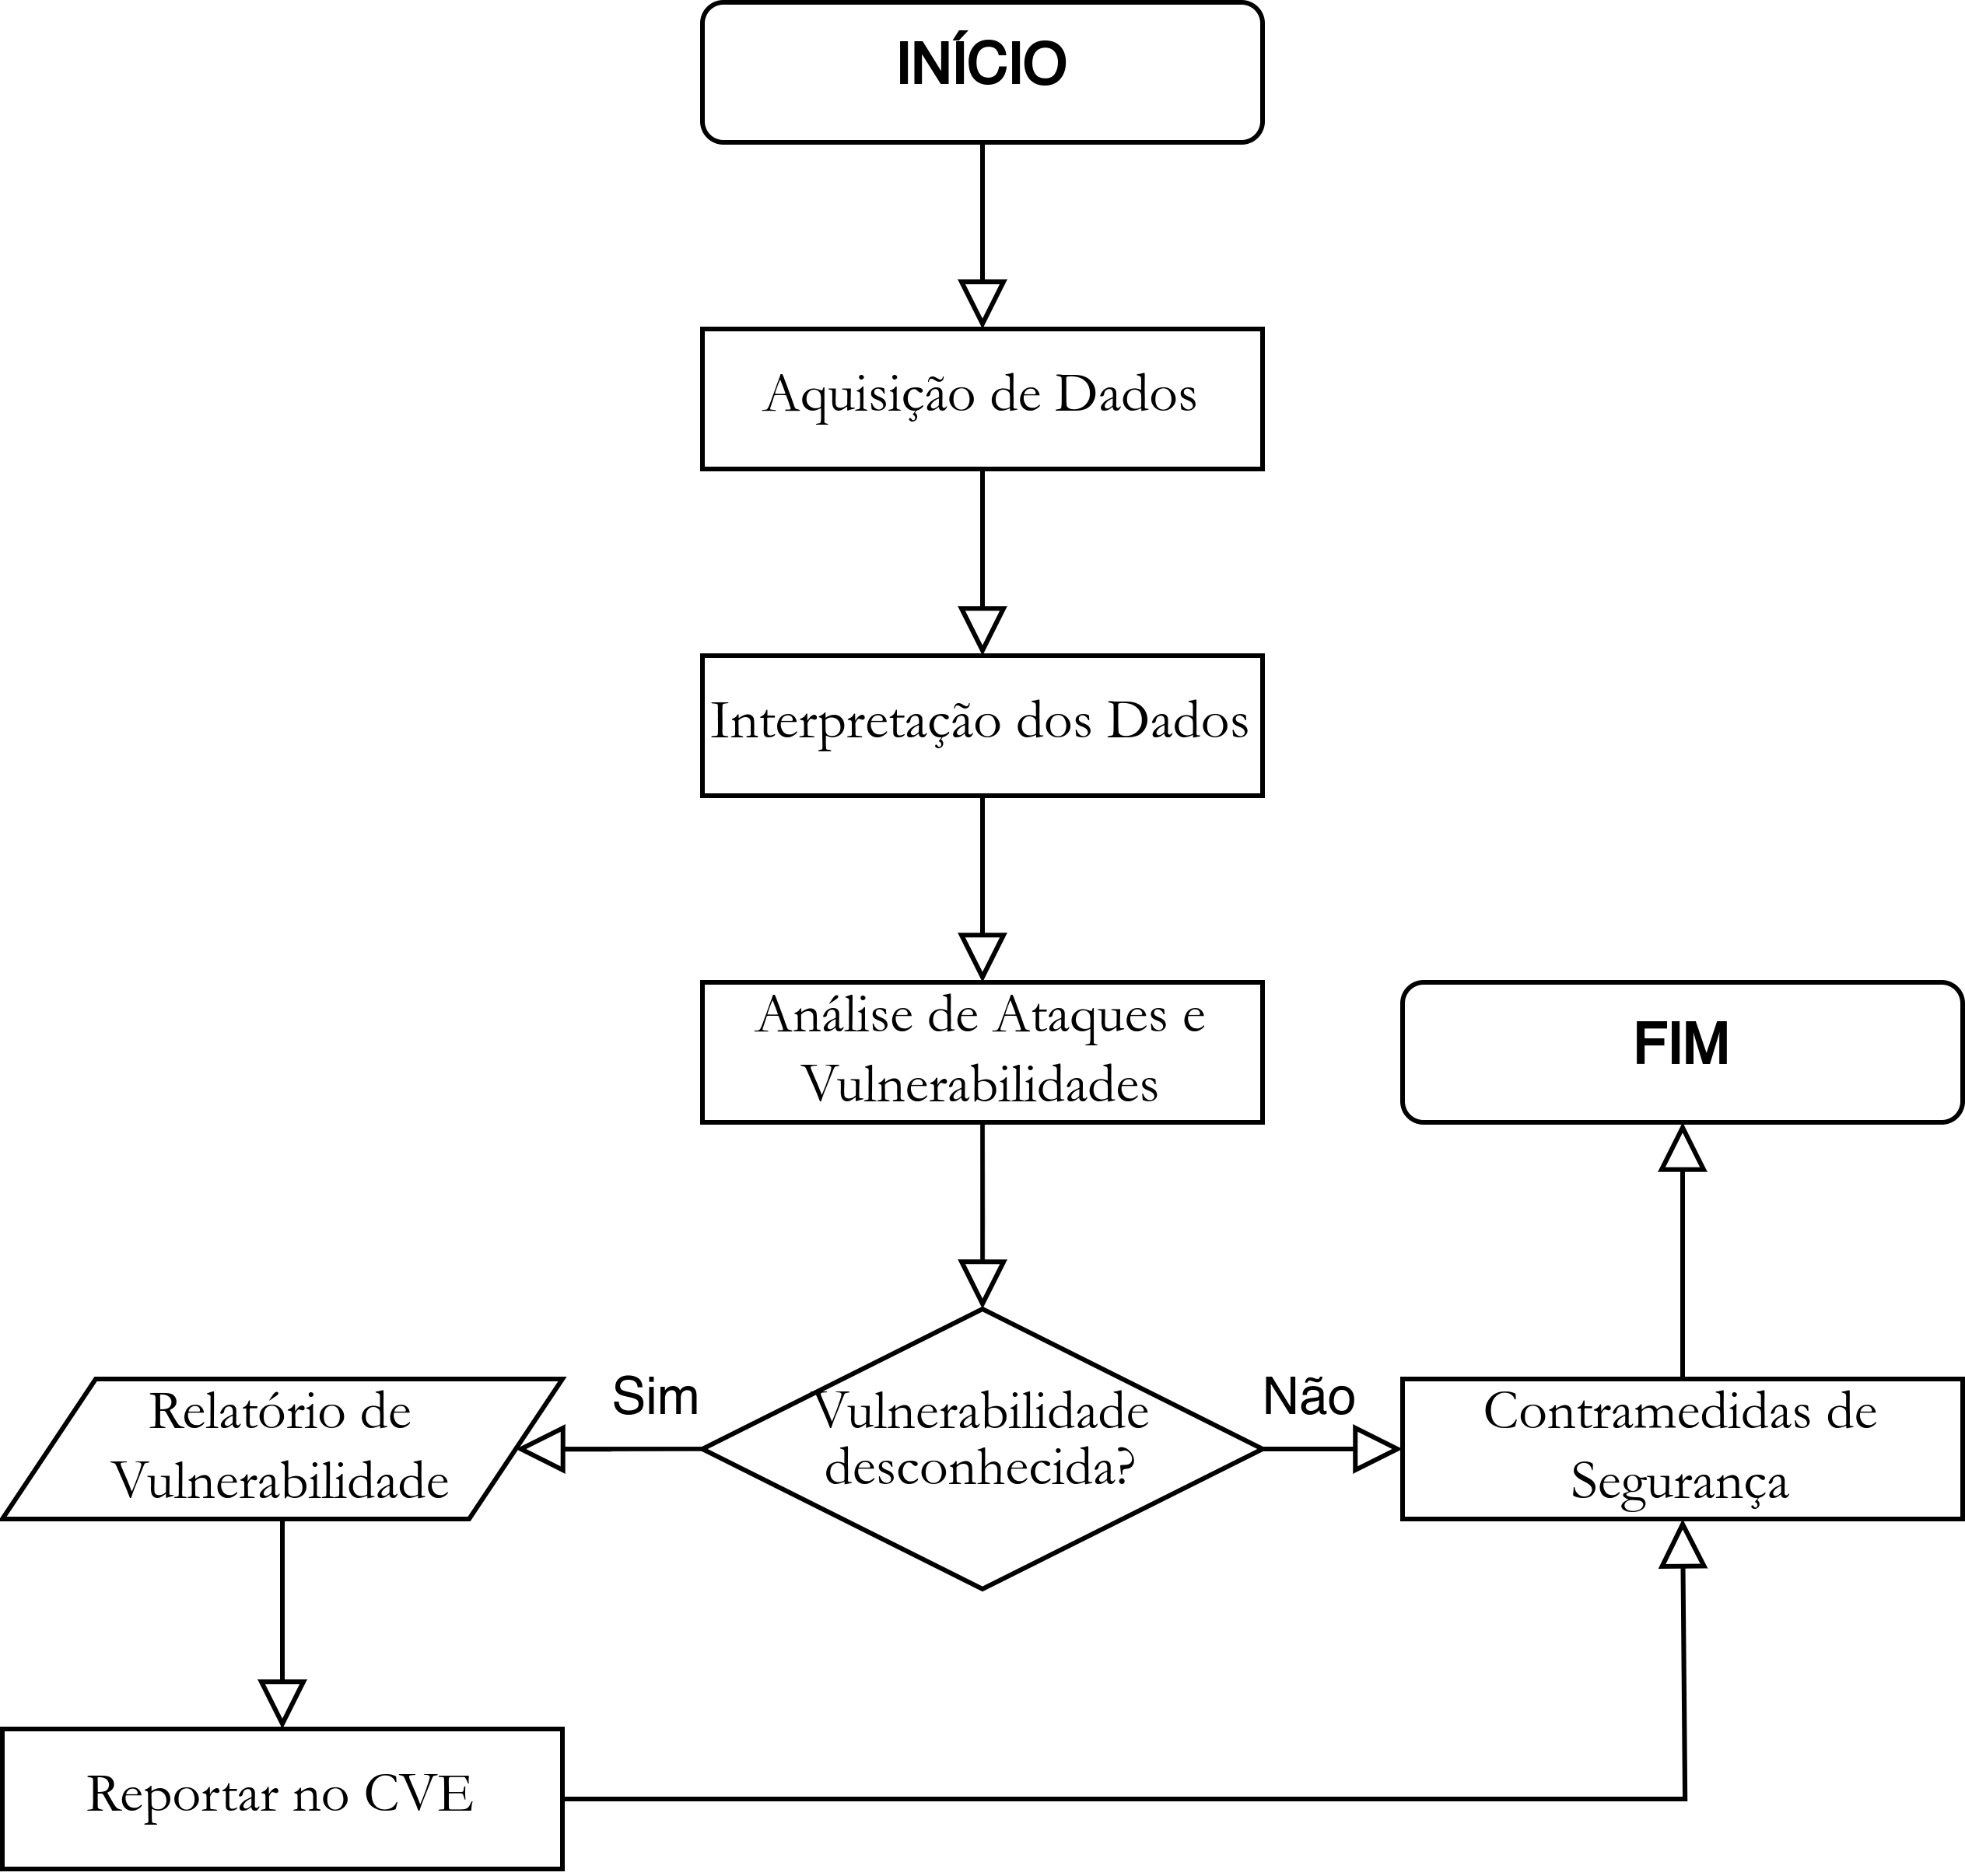
\includegraphics[width=0.7\textwidth]{USPSC-img/fluxograma.png}
        \end{center}
        \legend{Fonte: elaborada pelo autor.}
    \end{figure}

    Para a realização adequada do experimento proposto neste estudo, a infraestrutura de rede do protocolo OPC UA foi configurada conforme os seguintes parâmetros: o Raspberry Pi atuando como servidor e a DF63 NG desempenhando o papel de cliente. Além disso, um elemento de rede chamado `Sniffer' (conforme ilustrado na \autoref{fig:banc}) foi inserido na configuração para monitorar e registrar a comunicação da rede. Com o propósito de fornecer uma visão clara dos componentes envolvidos e facilitar a análise dos dados coletados durante o experimento, os endereços IP e MAC de cada elemento do sistema estão resumidos na \autoref{tab:ender}. Importante mencionar que o servidor OPC UA foram configurados para utilizar a porta padrão 4840, e os \textit{endpoints} correspondentes adotam o padrão abaixo. Essa estrutura de configuração foi essencial para a condução eficaz do experimento e a subsequente análise dos resultados.

    \begin{minted}[
        breaklines,
        %linenos,
        mathescape,
        encoding=utf8,
        framesep=2mm,
        baselinestretch=1.2,
        bgcolor=codeback,
        fontsize=\footnotesize
    ]{console}
<esquema>://<endereço>:<porta>/<DiscoveryEndpoint>
    \end{minted}

    Onde, `<esquema>' pode ser `opc.tcp' ou `opc.https', `<endereço>' é o endereço IP do servidor, `<porta>' é a porta de comunicação OPC UA, e `<DiscoveryEndpoint>' é o ponto de descoberta do servidor OPC UA.

    \begin{table}[htbp!]
        \centering
        \caption{Endereços IP e MAC dos equipamentos da rede OPC UA}%
        \label{tab:ender}
        \begin{tabular}{ccc}
            \toprule
            \thead{Equipamento} & \thead{IP} & \thead{MAC} \\
            \toprule
            DF63 NG  & 192.168.164.101 & 00:30:5C:24:13:66 \\
            \midrule
            RaspPi   & 192.168.164.102 & E4:5F:01:2E:1A:B6 \\
            % \midrule
            % RaspPi 2 & 192.168.164.102 & E4:5F:01:2E:1B:C1 \\
            \midrule
            Sniffer  & 192.168.164.201 & C8:3A:35:49:FD:58 \\
            \midrule
            Invasor  & 192.168.164.115 / 192.168.164.110 & 00:be:43:34:b8:54 \\
            \bottomrule
        \end{tabular}
        \fonte{elaborada pelo autor.}%
    \end{table}

    \subsection{Aquisição de Dados}

    A fase de aquisição de dados fundamenta-se na captura do tráfego de pacotes transmitidos pela rede OPC UA durante a comunicação entre a aplicação servidora e o cliente da rede, enquanto ocorrem os ataques. Esse processo se baseia na utilização do software Wireshark, no qual permite a coleta de informações cruciais sobre a comunicação, incluindo detalhes como o tipo de protocolo empregado, a origem e o destino dos dados. As informações capturadas são armazenadas em ordem cronológica com a capacidade de serem salvas em arquivos no formato `.pcapng'. O software Wireshark foi configurado para finalizar a captura com sessenta segundos de coleta.

    Os alvos dos ataques é o servidor OPC UA, e em cada cenário, o elemento \textit{Sniffer} é configurado para realizar a captura do tráfego gerado por estes ataques. Para organizar os pacotes capturados, foi adotada a seguinte nomenclatura de arquivos: `[Modo de Segurança]-[Tipo do Ataque]-[Número da Captura].pcapng'. Aqui, o modo de segurança pode assumir os valores 0 (None), 1 (Sign) e 2 (Sign\&Encrypt). Os tipos de ataques correspondem àqueles detalhados na \autoref{sec:attacks} (`sniffing', `mitm' e `dos-[função]'), e o número da captura é representado por um dígito de 0 a 9. Por exemplo, para salvar a terceira captura obtida durante uma negação de serviço pelo ataque de chamada da função \textit{Dereference} nula, com a rede configurada no modo de segurança \textbf{Sign}, o arquivo seria nomeado como: `1-dos\_function\_call\_null\_deref.pcapng'. A \autoref{tab:attacks} apresenta os arquivos de captura gerados durante os experimentos para cada tipo de ataque.

    \begin{table}[htbp]
        \centering
        \caption{Arquivos de captura gerados durante a fase de aquisição de dados}%
	    \label{tab:attacks}
        \begin{tabular}{lp{5cm}}
            \toprule
            \thead{Arquivo} & \thead{Ataque} \\
            \toprule
            (0/1/2)-dos\_certificate\_inf\_chain\_loop.pcapng & DoS pelo loop infinito na cadeia de certificados \\
            \midrule
            (0/1/2)-dos\_function\_call\_null\_deref.pcapng & DoS pela chamada da função \textit{Dereference} nula \\
            \midrule
            (0/1/2)-dos\_hping3.pcapng & DoS pela inundação do TCP/IP \\
            \midrule
            (0/1/2)-dos\_open\_multiple\_secure\_channels.pcapng & DoS pela abertura de múltiplos canais seguros \\
            \midrule 
            (0/1/2)-dos\_translate\_browse\_path\_call.pcapng & DoS pela tradução do caminho de navegação \\
            \midrule
            (0/1/2)-mitm\_arp.pcapng & MITM pela falsificação da tabela ARP \\
            \midrule
            (0/1/2)-mitm\_port.pcapng & MITM pelo roubo de portas \\
            \midrule
            (0/1/2)-sniffing.pcapng & \textit{Packet Sniffing} \\
            \midrule
            (0/1/2)-normal\_local\_server.pcapng & Comunicação normal entre cliente e servidor \\
            \bottomrule
        \end{tabular}
        \fonte{elaborada pelo autor.}%
    \end{table}

    % \begin{table}[htbp]
    %     \centering
    %     \caption{Arquivos de captura gerados durante a fase de aquisição de dados}%
	%     \label{tab:attacks}
    %     \begin{tabular}{ll}
    %         \toprule
    %         \thead{Arquivo} & \thead{Ataque} \\
    %         \toprule
    %         0-dos\_certificate\_inf\_chain\_loop.pcapng & \multirow{3}{*}{\parbox{6cm}{DoS pelo loop infinito na cadeia de certificados}} \\
    %         1-dos\_certificate\_inf\_chain\_loop.pcapng & \\
    %         2-dos\_certificate\_inf\_chain\_loop.pcapng & \\
    %         \midrule
    %         0-dos\_function\_call\_null\_deref.pcapng & \multirow{3}{*}{\parbox{6cm}{DoS pela chamada da função \textit{Dereference} nula}} \\
    %         1-dos\_function\_call\_null\_deref.pcapng & \\
    %         2-dos\_function\_call\_null\_deref.pcapng & \\
    %         \midrule
    %         0-dos\_hping3.pcapng & \multirow{3}{*}{\parbox{6cm}{DoS pela inundação do TCP/IP}} \\
    %         1-dos\_hping3.pcapng & \\
    %         2-dos\_hping3.pcapng & \\
    %         \midrule
    %         0-dos\_open\_multiple\_secure\_channels.pcapng & \multirow{3}{*}{\parbox{6cm}{DoS pela abertura de múltiplos canais seguros}} \\
    %         1-dos\_open\_multiple\_secure\_channels.pcapng & \\
    %         2-dos\_open\_multiple\_secure\_channels.pcapng & \\
    %         \midrule 
    %         0-dos\_translate\_browse\_path\_call.pcapng & \multirow{3}{*}{\parbox{6cm}{DoS pela tradução do caminho de navegação}} \\
    %         1-dos\_translate\_browse\_path\_call.pcapng & \\
    %         2-dos\_translate\_browse\_path\_call.pcapng & \\
    %         \midrule
    %         0-mitm\_arp.pcapng & \multirow{3}{*}{\parbox{6cm}{MITM pela falsificação da tabela ARP}} \\
    %         1-mitm\_arp.pcapng & \\
    %         2-mitm\_arp.pcapng & \\
    %         \midrule
    %         0-mitm\_port.pcapng & \multirow{3}{*}{\parbox{6cm}{MITM pelo roubo de portas}} \\
    %         1-mitm\_port.pcapng & \\
    %         2-mitm\_port.pcapng & \\
    %         \midrule
    %         0-sniffing.pcapng & \multirow{3}{*}{\parbox{6cm}{\textit{Packet Sniffing}}} \\
    %         1-sniffing.pcapng & \\
    %         2-sniffing.pcapng & \\
    %         \midrule
    %         0-normal\_local\_server.pcapng & \multirow{3}{*}{\parbox{6cm}{Comunicação normal entre cliente e servidor}} \\
    %         1-normal\_local\_server.pcapng & \\
    %         2-normal\_local\_server.pcapng & \\
    %         \bottomrule
    %     \end{tabular}
    %     \fonte{elaborada pelo autor.}%
    % \end{table}

    Além disso, é importante salientar que durante o processo de coleta de dados com o Wireshark, simultaneamente, obtêm-se informações sobre a carga de processamento da CPU nos hospedeiros do servidor OPC UA. Essa abordagem complementa significativamente a análise dos efeitos do ataque sobre o desempenho do sistema. Para viabilizar esse monitoramento, desenvolveu-se um \textit{script} que deve ser ativado pelo elemento \textit{Sniffer} no início da captura de dados.

    \begin{minted}[
        breaklines,
        %linenos,
        mathescape,
        encoding=utf8,
        framesep=2mm,
        baselinestretch=1.2,
        bgcolor=codeback,
        fontsize=\footnotesize
    ]{python}
import csv
import time
import os

def get_cpu_usage():
    """
    Calcula a utilização da CPU em percentual.
    """
    with open('/proc/stat') as stat_file:
        lines = stat_file.readlines()
    # Obtém os valores de CPU da primeira linha
    cpu_values = [int(val) for val in lines[0].split()[1:8]]
    # Soma os valores da CPU para obter o total de utilização da CPU
    total_cpu_time = sum(cpu_values)
    # Calcula a diferença entre a utilização da CPU atual e anterior
    delta_total_cpu_time = total_cpu_time - get_cpu_usage.previous_total_cpu_time
    delta_idle_cpu_time = cpu_values[3] - get_cpu_usage.previous_idle_cpu_time  # 4º valor é o tempo ocioso
    # Calcula a taxa de utilização da CPU em percentual
    cpu_percent = 100 * (1 - delta_idle_cpu_time / delta_total_cpu_time)
    # Atualiza os valores anteriores para a próxima iteração
    get_cpu_usage.previous_total_cpu_time = total_cpu_time
    get_cpu_usage.previous_idle_cpu_time = cpu_values[3]

    return cpu_percent

# Inicializa os valores anteriores
get_cpu_usage.previous_total_cpu_time = 0
get_cpu_usage.previous_idle_cpu_time = 0

def get_memory_usage():
    """
    Calcula a utilização da memória em percentual.
    """
    total_memory = float(os.popen("grep 'MemTotal' /proc/meminfo | awk '{print $2}'").read().strip())
    available_memory = float(os.popen("grep 'MemAvailable' /proc/meminfo | awk '{print $2}'").read().strip())
    used_memory = total_memory - available_memory
    memory_percent = (used_memory / total_memory) * 100
    return memory_percent

def main():
    """
    Função principal que realiza a coleta de dados de utilização da CPU e memória, e salva em um arquivo CSV.
    """
    output_file = '1-dos_hping3.csv'
    duration = 60  # Tempo de execução em segundos

    # Abre o arquivo CSV para escrita
    with open(output_file, mode='w', newline='') as file:
        writer = csv.writer(file)
        writer.writerow(['Timestamp', 'CPU (%)', 'Memory (%)'])

        start_time = time.time()

        while time.time() - start_time <= duration:
            timestamp = time.time() - start_time
            timestamp_str = '{:.6f}'.format(timestamp)
            cpu_usage = round(get_cpu_usage(), 2)
            memory_usage = round(get_memory_usage(), 2)

            writer.writerow([timestamp_str, cpu_usage, memory_usage])
            time.sleep(1)  # Captura de dados a cada segundo

if __name__ == "__main__":
    main()
    \end{minted}

    A implementação desta aquisição visa fornecer uma visão integrada do impacto dos ataques não apenas em termos de tráfego de rede, mas também em termos de uso de recursos do sistema, permitindo uma análise mais abrangente das vulnerabilidades e seus efeitos nas operações dos sistemas OPC UA. Esse monitoramento contínuo possibilita a identificação de padrões de comportamento anômalo que podem ser associados a atividades maliciosas, além de fornecer dados quantitativos que auxiliam na avaliação do impacto real dos ataques.

    Para garantir a precisão e a confiabilidade dos dados coletados, cada ataque foi repetido múltiplas vezes, e as capturas resultantes foram analisadas de forma comparativa. Esse método permite a identificação de variações nos resultados que possam ser atribuídas a fatores externos ou a inconsistências na execução dos ataques. Todas as capturas foram realizadas em um ambiente controlado, com a configuração dos dispositivos de rede e do servidor OPC UA mantida constante ao longo dos experimentos.

    \subsection{Interpretação dos Dados}

    Uma vez que o tráfego da rede é coletado para cada ataque e salvos nos arquivos de captura, os dados podem ser interpretados para o estudo de vulnerabilidades nos cenários propostos.  A análise detalhada dos dados capturados durante os ataques cibernéticos em redes OPC UA é fundamental para entender o impacto das vulnerabilidades exploradas. Assim, uma nova aplicação denominada \textbf{uanalyser} foi desenvolvida para auxiliar na interpretação dos dados capturados, permitindo a geração de gráficos específicos para cada cenário de ataque. A seguir, apresenta-se como os dados obtidos foram interpretados, destacando a importância dos gráficos gerados e a relevância da análise dos atributos monitorados.

    A geração dos gráficos visa fornecer uma representação visual dos principais indicadores de desempenho e segurança da rede OPC UA sob ataque. Logo, quatro gráficos são gerados para cada coleta: (a) \textit{Throughput} (kbps), (b) desempenho do hospedeiro do servidor OPC UA (RAM e CPU), (c) quantidade de pacotes OPC UA por segundo e (d) \textit{Round Trip Time} (RTT) normalizado, por pacote. Esses gráficos foram escolhidos devido à sua capacidade de ilustrar diferentes aspectos do funcionamento e da resiliência ou fragilidade da rede em condições adversas.

    Para a construção do \textbf{uanalyser}, utilizou-se a linguagem de programação Python e os seguintes pacotes essenciais para a obtenção dos resultados em gráficos: Scapy, Matplotlib, NumPy e Pandas, além de contar com os pacotes para o ambiente de desenvolvimento: MkDocs, PyTest e Taskipy.

    O Scapy é uma ferramenta poderosa para manipulação de pacotes de rede, que facilita a captura, a análise e a criação de pacotes, independentemente de pilhas predefinidas ou regras de rede comuns. Logo, utilizando os recursos desse pacote, o \textbf{uanalyser} lê arquivos de captura no formato .pcapng, extrai informações específicas dos pacotes e realiza análises detalhadas. O diagrama de sequência da aplicação é apresentado na \autoref{fig:seqUanalyser} e detalha como é realizada a interpretação destes dados. São construídos alguns gráficos que mostram como cada ataque afeta a rede em termos de \textit{throughput}, uso de recursos do hospedeiro, quantidade de pacotes por segundo e RTT.

    \begin{figure}[htbp!]
        \caption{\label{fig:seqUanalyser}Diagrama de sequência da aplicação \textbf{uanalyser}}
        \begin{center}
            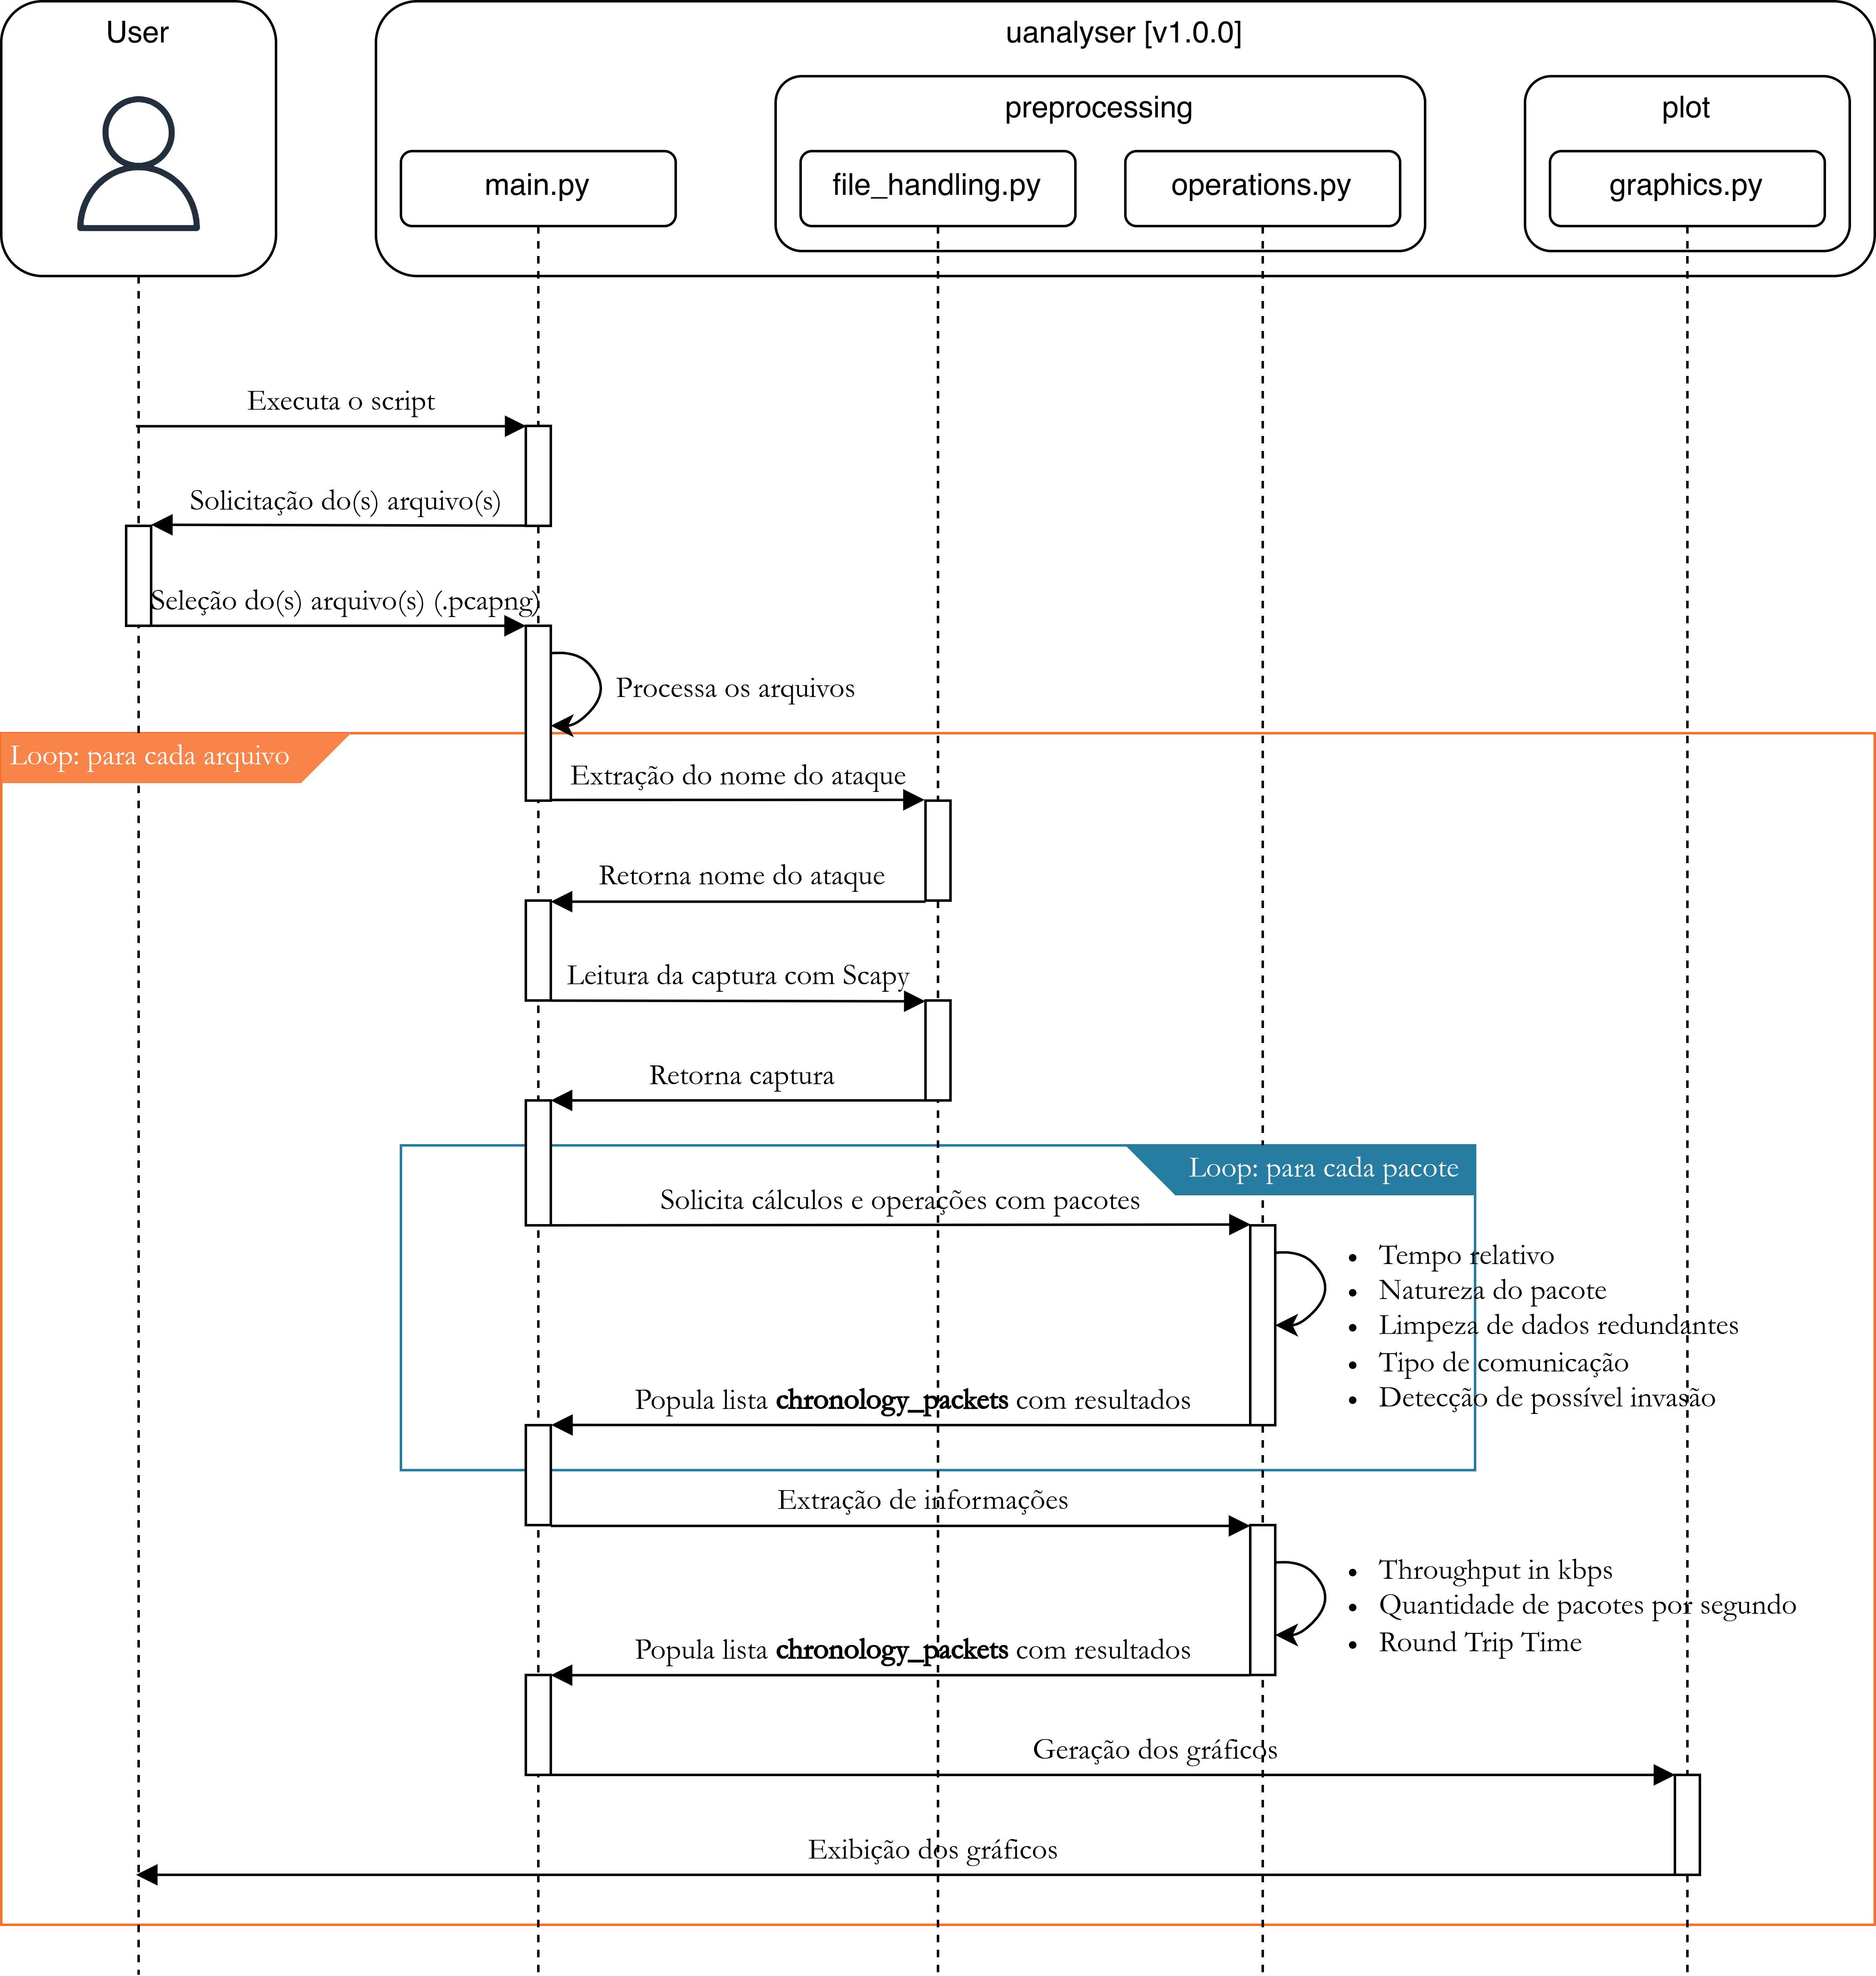
\includegraphics[width=0.972\textwidth]{USPSC-img/seqUanalyser.png}
        \end{center}
        \legend{Fonte: elaborada pelo autor.}
    \end{figure}

    Dentro do contexto do protocolo OPC UA, as mensagens trocadas entre cliente e servidor podem incluir várias estruturas de dados, como mensagens de sessão, mensagens de serviço e dados de publicação/subscrição. Cada tipo de mensagem tem seu próprio formato e estrutura, conforme especificado pelo padrão OPC UA. A análise dessas mensagens é crucial para identificar comportamentos anômalos e potenciais vulnerabilidades.

    A análise dos pacotes capturados e a visualização dos gráficos gerados pelo \textbf{uanalyser} permitem uma compreensão detalhada dos efeitos dos ataques nas redes OPC UA. Essa abordagem sistemática e visual facilita a identificação de vulnerabilidades específicas do protocolo e o desenvolvimento de contramedidas eficazes para melhorar a segurança e a resiliência das redes industriais.

    O software desenvolvido para este trabalho está disponível no GitHub \footnote{Disponível em: \url{https://github.com/JonathanTSilva/opcua-analyser}. Acesso em: 04 jul. 2024} e aberto para contribuições. Aqueles que desejarem contribuir devem seguir os padrões de desenvolvimento estabelecidos no arquivo \texttt{contributing.md} e aderir ao código de conduta do projeto.

    \subsection{Análise dos Ataques e Vulnerabilidades}

    A análise de ataques e vulnerabilidades em redes industriais OPC UA é um processo sistemático e detalhado que visa identificar, avaliar e mitigar possíveis pontos fracos no protocolo e na implementação de redes OPC UA. Esta etapa é essencial para garantir a segurança e a continuidade operacional dos IACSs e consiste na análise dos resultados da série de testes e simulações de ataques cibernéticos obtidos nos processos anteriores. Cada tipo de ataque explora diferentes vulnerabilidades potenciais do protocolo e da infraestrutura de rede.

    Ao testar vulnerabilidades da comunicação em redes industriais OPC UA, foca-se na determinação da qualidade da comunicação durante e após um ataque. Em outras palavras, se o equipamento é capaz de desempenhar sua tarefa nestes períodos. Adicionalmente, é examinado se o alvo sofre com falta de resposta ou respostas incomuns.

    Como a observação de soluções existentes faz parte da abordagem deste desenvolvimento, precisamos ter algum ponto de referência como base para nossas observações das vulnerabilidades existentes e comportamento durante ataques. Com base nisso, são definidas as seguinte classes de vulnerabilidades para este projeto em específico:

    \begin{itemize}
        \item \textbf{Classe 1}: falhas que interrompem o comunicação OPC UA entre os agentes, afetando a disponibilidade;
        \item \textbf{Classe 2}: serviços interrompidos ou comportamento inesperado que não alteram a comunicação, mas prejudica a integridade;
        \item \textbf{Classe 3}: vulnerabilidades que não interrompem a comunicação, mas afetam a confiabilidade.
    \end{itemize}

    A partir dos gráficos gerados e do comportamento da rede e dispositivos durante e após o ataque, é possível identificar as vulnerabilidades existentes e classificá-las de acordo com as classes supracitadas. Além disso, é possível verificar a eficácia das diferentes políticas de segurança do OPC UA (`None', `Sign', `Sign \& Encrypt'). A análise dos resultados obtidos é essencial para a identificação de possíveis falhas e a proposição de medidas corretivas e preventivas para mitigar os riscos de segurança nas redes OPC UA.

    Essa abordagem metodológica, que inclui a observação de gráficos de throughput, desempenho de RAM e CPU, quantidade de pacotes OPC UA por segundo e RTT normalizado, permite uma compreensão detalhada do impacto dos ataques nas redes industriais OPC UA. Com isso, é possível desenvolver estratégias de mitigação eficazes e assegurar a robustez e a resiliência das redes contra possíveis ameaças cibernéticas.
    
    \subsection{Relatório de Vulnerabilidade}

    A construção de um relatório de vulnerabilidade é uma etapa crucial no processo de avaliação de segurança cibernética, especialmente no contexto de redes industriais OPC UA. Através deste relatório, é possível documentar e comunicar as vulnerabilidades identificadas, fornecer uma análise detalhada dos riscos e propor contramedidas adequadas. Este documento é fundamental não apenas para entender as falhas de segurança, mas também para tomar ações corretivas eficazes e melhorar a postura de segurança da organização.

    A elaboração de um relatório de vulnerabilidade deve seguir padrões internacionais de segurança cibernética e estar alinhada com as melhores práticas do setor. Um bom relatório deve ser estruturado de forma clara e objetiva, contemplando diferentes níveis de detalhamento para atender a diversos públicos, desde executivos até equipes técnicas.

    O relatório de vulnerabilidade é essencial para diversos stakeholders dentro de uma organização. Ele auxilia os executivos a compreenderem a postura de segurança atual da empresa e a justificarem investimentos em segurança. Para a equipe de TI, o relatório oferece detalhes técnicos sobre as vulnerabilidades descobertas e orientações sobre como corrigi-las. Além disso, o relatório pode ser utilizado para fins de conformidade regulatória, sendo compartilhado com auditores e reguladores para demonstrar os esforços de segurança da organização.

    Para garantir a eficácia do relatório de vulnerabilidade, ele deve incluir as seguintes seções principais:

    \begin{itemize}
        \item \textbf{Sumário Executivo}: Uma visão geral de alto nível da avaliação, destinada a executivos não técnicos. Esta seção deve ajudar os executivos a avaliarem a postura de segurança da empresa e destacar quaisquer questões críticas que possam impactar a segurança corporativa ou a conformidade regulatória.
        \item \textbf{Visão Geral}: Uma seção voltada para um público mais técnico, fornecendo um resumo da avaliação. Deve incluir informações sobre os sistemas analisados, ferramentas utilizadas e o número e a severidade das vulnerabilidades descobertas.
        \item \textbf{Detalhes da Avaliação}: Esta seção deve fornecer detalhes técnicos sobre como a avaliação de vulnerabilidade foi conduzida. Deve descrever as etapas realizadas em cada fase da avaliação e seus resultados, permitindo que o leitor possa replicar os achados da avaliação.
        \item \textbf{Resultados}: Esta seção deve detalhar os achados da avaliação. As vulnerabilidades devem ser classificadas por severidade para chamar a atenção para os maiores problemas dentro do ambiente da organização. Para cada vulnerabilidade potencial verificada, esta seção deve descrever o resultado, os sistemas afetados, o nível de severidade e fornecer um link para informações adicionais, como um CVE.
        \item \textbf{Mitigações Recomendadas}: O objetivo de uma avaliação de vulnerabilidade é ajudar a organização a melhorar sua postura de segurança. Portanto, fornecer recomendações de mitigação é essencial. Em muitos casos, isso pode ser tão simples quanto recomendar uma atualização de software, uma senha mais forte em um sistema ou uma alteração em uma configuração de segurança insegura.
    \end{itemize}

    Uma vez que o relatório de vulnerabilidade é elaborado, ele deve ser aplicado nas bases de conhecimento da organização para garantir que todas as vulnerabilidades identificadas sejam tratadas de forma adequada. O relatório deve ser revisado regularmente e atualizado conforme novas vulnerabilidades sejam descobertas e medidas corretivas sejam implementadas. Além disso, é importante que o relatório siga os padrões globais de cibersegurança, como o CVE (do inglês \textit{Common Vulnerabilities and Exposures}) e os padrões de segurança IEC 62443, para garantir a consistência e a confiabilidade das informações.

    A utilização de frameworks reconhecidos internacionalmente, como o CVE e o IEC 62443, proporciona uma base sólida para a identificação e a classificação de vulnerabilidades. Estes padrões oferecem diretrizes claras sobre como avaliar e mitigar riscos, além de promover a adoção de práticas de segurança consistentes e eficazes. Além disso, existem diversos modelos para a elaboração de relatórios de vulnerabilidade, como o da CISA (Cybersecurity and Infrastructure Security Agency), do NIST (National Institute of Standards and Technology), que podem ser adaptados para atender às necessidades específicas de cada organização. Caso alguma vulnerabilidade desconhecida do protocolo OPC UA seja encontrada, será utilizado o modelo de relatório personalizado e disponibilizado no \autoref{ap:relatorio} para documentar e comunicar a descoberta.

    \subsection{Contramedidas de Segurança}

    Uma implementação bem projetada e sem complicações das contramedidas de segurança é uma das principais medidas para minimizar os riscos cibernéticos e maximizar a disponibilidade dos IACS. A segurança das redes industriais OPC UA deve contemplar uma abordagem holística, que inclua a proteção dos ativos de informação, a prevenção de ameaças e a detecção de incidentes.

    A determinação das contramedidas variam de acordo com o cenário de ataque e as vulnerabilidades identificadas. No entanto, algumas práticas comuns podem ser adotadas para fortalecer a segurança das redes OPC UA. Entre as principais contramedidas recomendadas estão:

    

    {\color{red}

    Análise de Vulnerabilidades Conhecidas:

    Utilizamos o banco de dados CVE para identificar vulnerabilidades conhecidas no protocolo OPC UA e em suas implementações. Cada CVE fornece detalhes sobre a vulnerabilidade, incluindo sua descrição, impacto e formas recomendadas de mitigação. Comparando essas vulnerabilidades com os resultados dos testes realizados, conseguimos correlacionar diretamente vulnerabilidades conhecidas com novas descobertas.

    Referência a Padrões de Segurança:

    Adotamos as diretrizes fornecidas pela norma IEC 62443, que é um conjunto de padrões desenvolvidos especificamente para a segurança de sistemas de automação e controle industrial. A IEC 62443 abrange desde os requisitos de segurança do produto até a gestão de segurança no ciclo de vida. Implementamos práticas recomendadas, como segmentação de rede, controle de acesso baseado em função e monitoramento contínuo de segurança.

    Frameworks Adicionais:

    Consultamos outros frameworks de segurança, como o NIST Cybersecurity Framework, para complementar nossas estratégias de mitigação com práticas amplamente aceitas e validadas. Integrando recomendações de múltiplos frameworks, criamos um conjunto robusto e abrangente de contramedidas.

    Implementação das Contramedidas
    Com base na análise das vulnerabilidades e nas diretrizes dos frameworks de segurança, implementamos as seguintes contramedidas:

    Melhorias na Configuração de Segurança do OPC UA:

    Criptografia e Assinatura: Reforçamos a criptografia e a assinatura digital para todas as comunicações OPC UA, conforme recomendado pelas políticas de segurança Sign e Sign \& Encrypt. Isso inclui a utilização de certificados robustos e algoritmos de criptografia atualizados.
    Autenticação Forte: Implementamos métodos de autenticação forte para acesso aos servidor OPC UA, incluindo autenticação multifator (MFA) e uso de certificados digitais para a autenticação de dispositivos.
    Segmentação de Rede e Controle de Acesso:

    Segmentação de Rede: Criamos zonas de segurança dentro da rede industrial para limitar a propagação de ataques. Cada zona é separada por firewalls e dispositivos de segurança que monitoram e controlam o tráfego de rede.
    Controle de Acesso Baseado em Função (RBAC): Aplicamos RBAC para limitar o acesso aos recursos de rede e serviços OPC UA apenas aos usuários e dispositivos autorizados, minimizando o risco de acessos não autorizados.
    Monitoramento e Resposta a Incidentes:

    Monitoramento Contínuo: Implementamos sistemas de monitoramento contínuo para detectar atividades anômalas e potenciais ataques em tempo real. Utilizamos IDS (Intrusion Detection Systems) e SIEM (Security Information and Event Management).
    Resposta a Incidentes: Desenvolvemos um plano de resposta a incidentes que define procedimentos claros para identificar, conter e remediar ataques cibernéticos. Este plano é baseado nas melhores práticas recomendadas pela norma IEC 62443 e frameworks de segurança correlatos.
    Fortalecimento da Infraestrutura:

    Atualizações Regulares: Garantimos que todos os componentes da rede, incluindo servidor OPC UA e dispositivos de rede, estejam sempre atualizados com os últimos patches de segurança.
    Hardening de Sistemas: Aplicamos técnicas de hardening para reduzir a superfície de ataque do servidor e dispositivos de rede. Isso inclui a desativação de serviços desnecessários, configuração segura de sistemas operacionais e aplicações, e implementação de políticas de segurança rígidas.
    Avaliação e Validação das Contramedidas
    A eficácia das contramedidas implementadas foi avaliada através de novos testes e simulações de ataques, utilizando o mesmo ambiente experimental. As principais atividades de avaliação incluíram:

    Reexecução dos Ataques:

    Realizamos novos testes de ataques cibernéticos sob as mesmas condições iniciais, mas com as contramedidas aplicadas. Isso permitiu a comparação direta dos resultados antes e depois da implementação das contramedidas. Monitoramos os indicadores de desempenho, como throughput, utilização de CPU e RAM, quantidade de pacotes por segundo e RTT, para verificar melhorias na resiliência da rede.

    Análise Comparativa:

    Comparamos os dados coletados durante os testes pós-contramedidas com os dados originais, para identificar reduções nos impactos dos ataques e melhorias na segurança da rede. Avaliamos a eficácia das contramedidas utilizando métricas de segurança, como a redução na taxa de sucesso dos ataques e o tempo de recuperação após incidentes.

    Feedback e Melhoria Contínua:

    Reavaliamos continuamente as contramedidas com base no feedback dos testes e na evolução das ameaças cibernéticas. Ajustes e melhorias foram implementados conforme necessário para garantir a proteção contínua da rede OPC UA.

    Conclusão
    A determinação e implementação de contramedidas de segurança em redes industriais OPC UA é um processo complexo, mas essencial para garantir a segurança e a integridade dos sistemas de automação e controle. Através da combinação de análise detalhada de vulnerabilidades, referência a frameworks de segurança reconhecidos e avaliação contínua da eficácia das medidas implementadas, é possível desenvolver uma abordagem robusta para proteger redes OPC UA contra uma ampla gama de ameaças cibernéticas. Este trabalho contribui para o fortalecimento da segurança nas redes industriais, promovendo a resiliência dos sistemas críticos em um cenário de ameaças em constante evolução.
    }